\documentclass[preprint]{aastex}

% TODO:
%   Add contours to images.

\usepackage{rotating}
\usepackage{amsmath}
\usepackage{graphicx}
\usepackage{xspace}

% some units
\newcommand{\mev}{\text{MeV}\xspace}
\newcommand{\gev}{\text{GeV}\xspace}
\newcommand{\tev}{\text{TeV}\xspace}
\newcommand{\sr}{\text{sr}\xspace}
\newcommand{\s}{\text{s}\xspace}
\newcommand{\ph}{\text{ph}\xspace}
\newcommand{\cm}{\text{cm}\xspace}
\newcommand{\tsext}{{\ensuremath{\text{TS}_\text{ext}}}\xspace}
\newcommand{\tsinc}{\ensuremath{\text{TS}_\text{inc}}\xspace}

\newcommand{\rsixeight}{{\ensuremath{\text{r}_{68}}}\xspace}

\newcommand{\tsextpointlike}{\ensuremath{\tsext_{,\pointlike}}}
\newcommand{\tsextgtlike}{\ensuremath{\tsext_{,\gtlike}}}
\newcommand{\tsextalt}{\ensuremath{\tsext_{,\alt}}}

\newcommand{\ts}{\text{TS}\xspace}
\newcommand{\glon}{\text{GLON}\xspace}
\newcommand{\glat}{\text{GLAT}\xspace}
\newcommand{\alt}{\text{alt}\xspace}

\renewcommand{\deg}{\ensuremath{^\circ}\xspace}

% the program names
\newcommand{\pointlike}{\text{\em pointlike}\xspace}
\newcommand{\python}{\text{\em python}\xspace}
\newcommand{\gtlike}{\text{\em gtlike}\xspace}
\newcommand{\gtobssim}{\text{\em gtobssim}\xspace}
\newcommand{\minuit}{\text{\em Minuit}\xspace}

\shorttitle{Search for Extended LAT Sources}

\begin{document}

\title{Search for Spatially Extended Fermi-LAT Sources Using Two Years of Flight
Data}

\author{
J.~Lande\altaffilmark{3}, 
\altaffiltext{3}{W. W. Hansen Experimental Physics Laboratory, Kavli Institute for Particle Astrophysics and Cosmology, Department of Physics and SLAC National Accelerator Laboratory, Stanford University, Stanford, CA 94305, USA}
}


\begin{abstract}
We present a new method for analyzing spatially extended sources with
the Fermi Large Area Telescope (LAT), the primary science instrument
on the {\em Fermi Gamma-ray Space Telescope (Fermi)}.  We provide a
series of Monte Carlo studies that were done to validate this tool.
We then calculate the Fermi LAT's sensitivity to spatially exnteded
sources.
We then apply this tool to test all sources in the 2FGL Two Year Catalog
for extension.\cite{2FGL} We then report on the discovery of XXXXXXXXXXXXXX new
extended sources.
\end{abstract}

\section{Introduction}

% * Resolving spatially extended Fermi sources is important for 
%    * studying supernova remnants, 
%    * pulsar wind nebulae, 
%    * galaxies,  
%    * potentially dark matter or new physics.
% * We searched all 2FGL catalog sources
% * Systematic test for a certain kind of (~ small) regularly shaped extended 

The Large Area Telescope (LAT) is a pair conversion telescope on the
Fermi Gamma-Ray Space Telescope. It has been surveying the Gamma-ray
sky since June 2008.  Fermi is particularly well suited as a survey
instrument because of its to survey the broad energy coverage ($20\mev$
to $>300\gev$), a wide field of view ($\sim 2.4 \sr$) and large effective
area ($\sim 8000 \cm^2$ at $>1\gev$).

Using one year of all sky monitoring, the LAT published a catalog of
source that were significantly resolved.  Many of these sources could
be be associated with a variety of source classes including active
galactic nuclei, pulsars, galaxies, and supernova remenants.  Many of
these source classes can be spatially resolved when observed at other
frequencies and could possibly be spatially resolvable by the LAT.

In particular, the LAT has discovered a variety of spatially extended
supernova remnants including IC443 and W51C (\cite{IC443,W51C}) and pulsar
wind nebulae (\cite{MSH15-52,VelaX}). And there are other source classes
which could possibly be spatially resolved by the LAT including galaxy
clusters, dark matter, and possibly new physics.

Furthermore, a variety of spatially extended but otherwise unassociated
sources have been detected in the galacitc plane at \tev energies using
Air Cherenkov detectors. Most prominent was a survey of the galaictc
plane using H.E.S.S which discovered XXXXXXXXX spatially extended
sources\cite{HESS_plane_survey}.

Being able to spatially resolve a fermi source is important for several
reasons. Most importantly, the spatial morphology can be used to help
identify a Fermi source. Because of the large point spread function (PSF),
for any source there are often several counterparts which it could be
associated with. Finding a matching morphology can uniquly identify the
source emitting the Gamma-rays. 

Because of the largely varying PSF of the LAT, the
spatial and spectral model of a source do not nicely decouple and
spatially resolving a Fermi source is also important for obtaining an
unbiased spectral model of the source.  Furthermore, using this extension
information is important for improved the overall model of the sky which
is important for obtaining a better fit of nearby sources and removing
spurious point sources which we might otherwise think we detect.


Nevertheless, morphological studies of sources in the $\gev$ energy range using
the Fermi LAT is challenging because of the significantly energy
dependent PSF and because of systematic errors in the
galactic diffuse emission. The Fermi PSF varies from over $XXXXXXXXXXXXXXX\deg$
at $100\mev$ to $XXXXXXXXXXXXXXXX\deg$ at $100\gev$ so the higher energy photons 
are significantly more important for resolving a source. On the other hand, 
we tend to run out of photons at higher energies so a detailed statistical 
test must be used to maximize our sensitivity.

\section{Analysis Method}


%   * Difficulty of studying spatially extended sources
%   * Pointlike, great features
%   * modifying it to fit spatially extended sources.
%      * semi-analytic convolution formula
%   * importance of fitting position + extension + spectrum simultaneously to apply statistical significance
%   * Monte Carlo Validation
%

Performing morphological studies of sources in the $\gev$ energy range using
the Fermi LAT is challenging primarily because of the significantly energy
dependent PSF and because of systematic errors in the
galactic diffuse emission. The Fermi PSF varies from over $XXXXXXXXXXXXXXXX\deg$
at $100\mev$ to $XXXXXXXXXXXXXXXX\deg$ at $100\gev$ and so the higher energy photons are
significantly more important for studying the shape of sources. One could
ideally look at just the highest energy photons, but the trade off is that
for typical sources many more source events are expected at low energy.
For this reason, it is especially important to use as much of the data
as possible.

The second primary difficult in studying spatially extended sources is
systematic uncertainties in the diffuse emission. Systematic errors are
notoriously difficult and will be discussed more later, but the important
point to make here is that one of the most important diagnostic tools for
studying systematic errors is being able to iterate the analysis while
varying different parameters such as what goes into the diffuse model.

\subsection{The \pointlike Package}

A new analysis tool has been developed to address these unique
requirements for studying spatially extended sources with the Fermi
LAT. The overall approach for this analysis is to perform a maximum
likelihood analysis where the Poisson likelihood for observing the
measured counts is computed given an assumed sky model. The parameters
of the sky model are then fit by maximizing the log of the likelihood.
To study the extension of a source, one can assume a particular shape
for an extended source (e.g. a disk or Gaussian), and fit the spatial
parameters of that source.

In principle, the entire task can be done using the standard science
tools package \gtlike\cite{Science-Tools-gtlike}. But \gtlike is
only able to fit the spectral parameters of the source, so the extension
fitting would have to be done as an external loop. Typically, the run time
for a binned source analysis using \gtlike is several hours so this loop
would be especially time consuming. In principle, parallel computing could
ease this burdon, but parallel fitting algorithms are rather untested
and complex. Furthermore, the machinery required to do something like
this would necessarily be rather complex. What has typically been done by
the Fermi team to study extended sources is to fix the assumed position
of the extended source, either by our knowledge of a source from other
wavelenghts, or by fitting it as a point source. Then, a profile of the
likelihood as a function of extension is developed using \gtlike
and the maximum of this profile. This approach is not optimal because it
needs not be the case that the best fit position of a point source would
be the same as the best fit position of an extended source. Furthermore,
by not fully maximizing the likelihood, this method is not as significant to
extension, especially of faint sources. And finally, since this approach
is so computationally intensive, no large scale Monte Carlo effort has been
launched to validate the method.

Instead, an alternate approach was developed for performing
a morphological analysis. An alternate maximum likelihood fitting
package called \pointlike has been developed by the Fermi
collaboration and we have expanded its functionality to fully support
analyzing spatially extended sources. \pointlike is most thoroughly
described in Matthew Kerr's Ph.D Thesis\cite{matthew_kerr_phd_thesis}
but the important aspects will be summarized below. What differentiates
\pointlike most significantly from \gtlike is its emphasis
on speed by introducing approximations into the calculation of the
likelihood function while at the same time trying to reduce any
numerical errors that may be introduced.  Like binned \gtlike,
\pointlike bins the sky both in position and energy.  Unlike 
\gtlike, \pointlike relies on the {\em healpix} representation of spatial
bins\cite{healpix_paper} and scales the size of each spatial bin to be
smaller than the PSF. This is convenient because it no
significant information is lost due to binning at all energies and it is
always a good approximation that the model predicted counts are uniform
across a spatial bin. 

\pointlike additionaly bins the Fermi Gamma-rays by their conversion
type, which corresponds to whether the photon converted in the front or
back part of the detector. Since the PSF is smaller for front entering
events, one would expect binning each conversion type independently to
improve our sensitivity.

Furthermore, \pointlike uses a sparse matrix representation of the spatial
bins where only the bins with counts in them are looped over. The only
downside to this is that the integral of the model predicted counts
must be independently calculated.  Effectively, \pointlike efficiently
interpolates from a totally binned analysis at low energy (where the
resolution is poor and there are many counts) to an unbinned analysis
at high energy (where the resolution is very good but there are few
counts). This approach provides a significant savings in time while
introducing only small numerical error.

Finally, \pointlike is written mostly in the \python programming language
using numpy and scipy to vectorize most of the computations. This provides
a reasonable tradeoff between computational efficiency and quickness
of development time. And by leaving the interface to use \pointlike as a
series of \python modules, advanced functions including extension fittion
described in section~\ref{extesion_fitting} and the dual localization
procedure described in section~\ref{dual_localization_method} could
quickly be build on top of the core modules.

\subsection{Extension Fitting}
\label{extension_fitting}

We have modified \pointlike to support fitting spatially extended
sources.  To do this, we introduced a new class of diffuse sources where
the spatial and spectral information completely decouple and where
the spatial shape is parameters by simple shapes.
The code consistently convolves the extended source shape with the point
spread function (as a function of energy) and integrates the spectrum over energy
to computed model predicted counts.

Finally, \pointlike allows the spatial parameters of an extended
source to be simulataneoulsy fit. \pointlike uses the \minuit fitting
library to perform the maximum likelihood maximization of the position
and extension of an extended source (\cite{minuit_documentation}).  At each
step in the fit of the shape, the spectral parameters of the entire sky
model are reoptimized. To avoid projection effects, what is directly
fit is not the longitude and latitude of the source but instead
the displacement in a rotated reference frame. 


\pointlike optimizes the analysis of extended sources in two ways.
First, for extended sources which are radially symmetric, the convolution
of the source shape with our parameterization of the PSF can be performed
semi-analytically. Generally, at a given energy the observed 
photon distribution is
\begin{equation}
  \text{PDF}(\vec r) = \int  \text{PSF}(|\vec r - \vec r'|)I_\text{src}(\vec r') d A' 
\end{equation}
where $I_\text{src}$ is the extended soruce shape and the PSF is parameterized by
\begin{equation}
  \text{PSF}(\vec r) = 
  \frac{1}{2\pi\sigma^2}
  \left(1-\frac{1}{\gamma}\right)
  \left(1+\frac{u}{\gamma}\right)^{-\gamma}
\end{equation}
Here, $\sigma$ and $\gamma$ are parameterize the $PSF$.
If the extended source is radially symmetric, then
$I_\text{src} (\vec r') = I_\text{src} (r')$ and the angular part of the
integral can be done analytically, leaving a simpler one dimensional
integral:
\begin{equation}
  \text{PDF}(u)= \int_0^\infty dv
  I_\text{src}(v) 
  \left(\frac{\gamma-1}{\gamma}\right)
  \left( \frac{\gamma}{\gamma + u + v}\right)^\gamma 
  \times ~_2F_1 \left(\gamma/2,\frac{1+\gamma}{2},1,\frac{4uv}{(\gamma+u+v)^2}\right)
\end{equation}
Not only is this convolution formula faster, but it has the advantage
that it more accurately reduces to the actual PSF shape as the source's
size decreases.  Decreasing the numerical difference between a small extended
source and the PSF is important when searching for smaller extended sources
and when determining the statistical significance of a detection.

There is one final approximation which speeds up the convolution.
Generally, the PSF is a function of the angle $\theta$ of the incident
event measured relative to the normal to the LAT. To avoid repeatedly
convolving the source shape with the PSF at a series of $\theta$ angles,
an effective PSF is fit to the weighted sum of the PSF times the exposure
at different $\theta$ angles.  Since the source convolution has to be
done at each fit iteration, these optimization were essential for making
this tool fast enough for the following analysis. Typically, the entire
process of fitting the extension and estimating the errors for a source
would run on the order of an hour.

\subsection{Extension Errors}

Errors on fit parameters are typically calculated in one of two ways. The
first method requires explicilty varying one paramter until the log of
the likelihood has fallen by a value 1/2 while simulatenously optimizing
the other fit parmaeters.  \minuit provides the {\em Simplex} function to
calculate errors this way.\cite{minuit documentation and UP parameter}
The second method involves estimating the likelihood function as being
a multivariate gaussian and calcluating the curvature of the log of
the likelihood at the peak to estimate when the function will fall by
a value 1/2. \minuit provides the {\em HESSE} algorithm to calcualte
errors this way.  The {\em HESSE} are significantly faster but make the
approximation that the log of the likelihood is perfectly gaussian.

We found that although much faster, the {\em HESSE} algorithm would
somtimes grosely understimate the errors on the localization and extension
of the source.  On the other hand, we found the {\em Simplex} algorithm
was computationally very slow and would often run into convergence
problems and fail to get reasonable errors.

As a compromise, we employed a hybrid approach to calculate
the localization and extension errors in \pointlike by making the
approximation that the covariance between the extension and location of
the source was small. On the other hand, we do not necessarily expect the
likelihood profile to be Gaussian when varying the source's extension.
So we calculate the error on the extension by fixing the position of the
source and then explicitly using {\em Simplex} to vary the extension of
the source until the log of the likelihood has fallen by 1/2.

Then, the extended source's position error is calculated using the
same code employed to calculate position errors of point sources. This
code is used to calculate the localization error of all point sources
in the catalog\cite{2FGL paper}. It works by fitting an ellipse to the
likelihood surface near the maximum and using this fit ellipse to estimate
an elliptical localization errors. By reporting two localization errors
as well as a localization error angle, this method explicitly takes care
of covariance between the two position coordinates.


% Make an extension profile plot.
% show it in figures an ddescirbeit.

\subsection{Gtlike Crosscheck}

Because of its computational speed, \pointlike is especially well
optimized for analysis that requires many iterations. This include
source localization, extension fitting, source finding, building test
statistic maps, and model comparison. On the other hand, \pointlike's
efficiency has to entail some loss of precision and so it is generally
expected that \gtlike will produce a more precise result.  Furthermore,
because it is the standard likelihood analysis package, \gtlike has been
more extensively validated and is very well trusted.

For that reason, we take our best fit source model obtained by
\pointlike with the best fit positions and extensions and refit the
spectral parameters of the model using \gtlike.  \gtlike provides a
second calculation of the likelihood which can then be used to obtain
for any source a second measure of \ts and \tsext.

We find very good agreement between the two methods. For the new extended
source candidates, Table \ref{alt_diff_model_results} shows a comparison
of \ts and \tsext computed using \pointlike and \gtlike. For the rest
of this paper, unless otherwise mentioned all \ts, \tsext, flux, and
spectral index values were obtained using \gtlike with the localization
results found by \pointlike.

\subsection{Dual Localization}
\label{dual_localization_method}

There is a degeneracy in the signal expected from spatially extended
sources and multiple point sources.  To assess the possibility of source
confusion, we developed a function in pointlike for simulatenously fitting
two point sources so that the likelihood fitting two point sources
could be compared to the likelihood fitting one extended source.

The algorithm works by first dividing the selected point source into
two separate sources. Then, the position of the two sources 
are fit simultanously. To avoid projection effects, the fit is
done in a coordiante system rotated to the celestial equator.
In this rotated coordiante system, space can be well approximated
as being flat and we are interested in fitting the 
rotated coordiante $(x_1',y_1')$ and $(x_2',y_2')$
We decided not to directly fit the positions of the two sources 
but instead the fit sum and difference of the rotated coordiantes
$S_x=(x_2'+x_1')/2$, $S_x=(y_2'+y_1')/2$, $D_x=(x_2'-x_1')/2$, and $D_y=(y_2'-y_1')/2$.
We believe that fitting the average of position and the difference
independently would cause less degeneracy in the fit and help the fitter
find the best position.

For a particular value of $S_x$, $S_y$, $D_x$, and $D_y$, the Poisson
likelihood is computed by converting the sum and difference coordinates
into the rotated coordiantes, unrotating the coordiantes, moving the
two sources in the \pointlike to the new positions, and performing a new
spectral analysis at the modified position.  The function then maximizes
The Poission likelihood $L(S_x,S_y,D_x,D_y)$ as a function of the sum
and difference of the rotated coordaintes using the Minuit to fit the
sum and differenc coordiantes (\cite{minuit_documentation}).

After the minimization converges, we can define the parameter $\tsext$
as twice the increase in log likelihood between fitting the region with
two point sources and fitting the region with one point source
\begin{equation}
  \tsext=2\times(LL_\text{ext}-LL_\text{ps}).
\end{equation}
Generally, \tsinc can be directly compared to \tsext to see wheter two
point sources are prefered over one extended source. Unfortunatly,
performing a likelihood ratio test between two unnested models
is not a calibrated test and so there is no straightforward way
to convert the change in likelihood into a significance~\ref{
http://arxiv.org/abs/astro-ph/0201547 }. Nevertheless, we find this
ratio, at least in the extreme case where $\tsinc \ll \tsext$ or
$\tsinc\gg\tsext$ to be suggestive. For all the spatally extended
candidates found, we computed both \tsext and \tsinc.

Because of \pointlike's computational efficiency, this algorithm
runs in a reasonable amount of time.

\subsection{Comparing Source Sizes}

% XXXXXXXXXXXXXXX This section needs work

When running \pointlike, we have to pick a spatial model for an extended
source. Our spatial model is then convolved with the PSF to create the
probability density function (PDF) that is is fit to the obersved counts.
Possible choices for spatial models include a Two dimensional gaussian
source (defined as a Gaussian in $x$ times a Gaussian in $y$):
\begin{equation}
  \text{PDF}(x,y)=\tfrac{1}{2\pi\sigma^2}\exp\left(-(x^2+y^2)/2\sigma^2\right)
\end{equation}
or a uniform disk:
\begin{equation}
  \text{PDF}(x,y)=\tfrac{1}{\pi\sigma^2}\delta\left(\sqrt{x^2+y^2}<\sigma\right).
\end{equation}

Although these shapes look significantly different from eachother, the
convolution of these spatial models of typtical sizes 
with the PSF will produce PDFs that are very similar.

This is demonstrated in figure~\ref{compare_disk_gauss}.  The plot shows
(in black) the PSF that would be observed for a source of spectral index
2. The dashed red (blue) line shows the probabability density function
for a Gaussian (uniform disk) of width $0.5\deg$.  The solid red (blue)
line shows the probability density function for the same Gaussian (uniform
disk) convolved with the PSF of an index 2 source.  
figure~\ref{compare_disk_gauss} shows the analysis using an energy range
of 1\gev to 100\gev whereas the right plot shows an analysis using an
energy range from 10\gev to 100\gev.

This plot shows that significantly different extended source shapes
look very similar after smearing with the PSF. The convolved shape of
the disk and Gaussian admittedly do look more different when restrict
ourselves to higher energy where the PSF is narrower, but we do not
excpet to have much luch learning about the exact nature of the
extended source shape. For that reason, in this paper we always use
the uniform disk spatial model to emphaizie our ignorance to the true
shape of the extended sources we are studying.

To get the convolved disk and Gaussian models looked so similar in
figure~\ref{compare_disk_gauss}, we had to pick the extension of the two
sources so that they each predicted a 68\% containment radius of 0.5\deg.

The 68\% containment radius for a spatial model is
the radius at which 68\% of the intensity is enclosed.
It can be computed by a straightforward integral and we
find that $\rsixeight_\text{,disk}=0.82\sigma$ whereas
the $\rsixeight_\text{,Gaussian}=1.51\sigma$. Therefore, in
figure~\ref{compare_disk_gauss} the uniform disk has an extension
of $\sigma=0.41\deg$ whereas the Gaussian has an extension of
$\sigma=0.75\deg$. Even though these sources have quite different
values of the extension $\sigma$, they look almost identical when convolved
with the PSF.

Finally, we note that comparing observed morphologies to 
counts maps can be misleading.  This effect can best be seen
in figure~\ref{compare_r68} where we have simulted a
extended source with 
a spatial model that is a uniform disk of extension 0.5\deg,
integral flux between 1\gev and 100\gev of $3e-8\ph/\cm^2/s$,
and a spectral index of 2. 

To reduce Poisson noise, figure~\ref{compare_r68} shows a counts map of
this simulated source smoothed with a 0.1\deg Gaussain kernel.  Overlaied
on the plot is the results of fitting this simulated source with a uniform
disk and a Gaussian spatial model.  The solid white line represents the
fit extension $\sigma_\text{disk}=0.496$ for the disk which was found to
be in very good agreemen with the simulated value.  The solid black line
represenst the fit extension $\sigma$ for the Gaussian which was found to
be $\sigma_\text{Gaussian}=0.2627$.  The white dashed line is the 68\%
containment radius of the fit Disk shape and the black dashed line is
the 68\% containment radius of the fit Gaussian shape.  Even though the
fit $\sigma$ for the disk and uniform Gaussian are different, the fit
68\% continment radius are very similar ($\rsixeight_\text{,disk}=0.41$
whereas $\rsixeight_\text{,Gaussian}=0.40$).

There are three important conclusions to take from this. The first is
that depending upon what spatial model you pick and what parameter you
choose to overlay on the smoothed counts ($\sigma$ or $rsixeight$),
you will get very different looking shapes even though the all lead
to a PDF which is very similar. And since we are not very sensitive
to the particular morphology of extended sources that we are seeing,
there is no correct choice for which shape to use. For the following
analysis, we always use a uniform disk as our spatial model because
of its conceptual simplicity and to emphasize our ignorance to the
true morphology. And for subsequent smoothed counts maps, we overlay
the $\sigma$ because that shows directly the edge of the shape we fit.
But due to smearing of the PSF, it has the unfotunatly concequence that
the extended source shape always (including in the simulated image)
looks larger than in the counts map.

The second conclusion we make is that because a counts map is smeared
out by the PSF and depends strongly on the particular color bar used, it
is very difficult to determine directly from a counts map a reasonable
spatial model that fits the data.  It is much better to obtain the
spatial model by a direct fit of a spatial parameters of a selected
model to the data.  The third conclusion we make is that when comparing
fit extensions to those at other wavelenghts (espeically in \tev), it is
important to compare fits of consistent spatial models. If this is not
possible, it is impotant to at least compare indirectly the $rsixeight$
for the different spatial models.


\section{LAT Extended Source Validation}

\subsection{Significance of Extension}

To calculate the statistical significance of the extension of a source,
one can define a parameter $\tsext$ as twice the increase in log
likelihood between fitting a source with a spatially extended hypothesis
and a point hypothesis:
\begin{equation}
  \tsext=2\times(LL_\text{ext}-LL_\text{ps}).
\end{equation}
Of course, these are nested hypotehsis since a point sources is just an
extended source in the limit that the extension goes to 0. So since we
are just adding a paramter, it should always be true that $\tsext > 0$
We would expect that if we were really testing a point source that
\tsext would not be very large since a point model would fit about
as good as anytthing else. Therefore, we can consider a source to be
extended (and reject the null hyopthesis) if \tsext is large enough.
Since going from fitting a point soue to fitting a simple extended
source introduces only one degree of freedom (the source's extension)
Wilks' Theorem says that the distribution of $\tsext$ wen testin
point sources should follow a $\chi^2_1$ distribution with one degree
of freedom (\cite{wilks_theorem}).

On the other hand, since the null hypothesis rests on the edge of
parameter space, when the extension is fixed to 0, Wilks' Theorem does
not formally hold (\cite{warn_wilks_theorem}).  One might
expect the actual distribution to be a half $\chi^2_1$ distribution with
one degree of freedom plus half of a delta function at 0:
\begin{equation}
  P(\ts)=\tfrac{1}{2}(\chi^2_1(\ts)+\delta(\ts)).
\end{equation}
Chernoff proved that given certain assumtipons, this is
the ditribution that would hold when the null hypothesis
lies on the edge of parameter space for a particular parameter~\ref{chernof}.
The false detection probability can be estimated by integrating this function 
from an observed test statistic value to infinity. It is for this
particular distribution that the often quoted result holds that
$\sqrt{\ts}$ is a measure of the number of $\sigma$ of the detection.

It should be noted that Wilks' Theorem only holds when the likelihood
is maximized simultaneoulsy fitting all of the parameters of model. It
is for this reason why \pointlike goes through such great effort to
simultaneously fit the position, extension, and spectral paramters of
a source.

The half $\chi^2_1$ distribution was found by a monte carlo study
to hold for the special case of source finding of EGRET sources using the
maximum likelihood technique.  They were comparing the hypothesis of a
source to the hypothesis of just a background\cite{Mattox_et_All_Paper}.
Their argument for why this null hypothesis distribution was reasonable
was that half of the time, statistical underfluctuations would cause
there to be fewer fewer photons then expected where the sources is being
tested. Since the maximim likelihood machinery cannot fit negative
sources (which would lead to negative model predicted for which the
poisson likelihood is undefined), half of the tests would not have the
likelihood improved by adding a source to the model and $\ts=0$.
It is for the case that the null distribution has 

It seems plausable that a similar situation could happen when testing
a source for extension. Half of the time, statistical flucutations might
make the observed counts narrower thant the point spread function and
the likelhood would not improve by fitting the source with an extended
hypothesis. We tested this hypothesis below using a dedicated monte
carlo study.

One issue that we found when testing this analysis method is that
despite our best efforts, there was always a small discrepancy between
the likelihood value when fitting the source as a point source and when
fitting it as an extended source with a small extension.  This is to be
expected due to numerical innacuracies introduced by the convolution.
For most cases, this error is insignificant. It would not significanlty
bias any of the fit values or errors. But it would bias the distribution
of $\tsext$ in the null hypothesis. To correct for this,
instead of computing the likelihood in the null hypothesis by fitting
a point source, a new source model was introduced which is an extended
source with its extension fixed to a very small value. $LL_\text{ps}$
is then calculated by refitting this source using the same extended
source fitting code. It was only after introducing this change that we
were able to get broad agreement between simulations and Wilks' theorem.


\subsection{Monte Carlo Validation} \label{monte_carlo_validation}

We performed a dedicated monte carlo study to validate \pointlike for
studying spatially extended sources and also to demonstrate that we can
use $\tsext$ as a test of the statistical significance
of a source's extension.  The monte carlo study involved simulating point
sources of varying spectral models on top of a simulated background. The
simulated point source was then fit using \pointlike as both an extended
source and a point source and $\tsext$ was calculated.

Fermi LAT data was simulated using the publically avaliabable Science
Tools package \gtobssim\cite{GTOBSSIM_CITATION}. The sources were
simulated with a powerlaw spectral model with 6 Were given 6 $>100\mev$
fluxes ranging from $3\times 10^{-9} \ph/\cm^2/s$ to 
$10^{-6} \ph/\cm^2/s$.
The sources were then simulated with spectral index ($\gamma$) values of
1.5, 2, 2.5, and 3.  These values were picked to probe a representative
range measurable values.  For particular spectral indices, only the
fluxes which would create a statistically significant source detection
($\ts>25$) where selected, since we are only interested in
testing for extension sources with a significant extent. The sources were
simulated on top of an isotropic powerlaw background with a Sreekumar-like
spectrum ($>100\mev$ flux of 1.5e-5 and spectral index 2.1).\cite{Sreekumar
et al. ApJ 494 pag 523 1998}

The monte carlo simulation was perforormed over a one year time interval using
a default rocking profile and an assumed a represntative
livetime fraction of 0.8.
The reconstruction was perfromed with events from an energy range of
$1\gev$ to $100\gev$ using 4 energy bins per decade and using the Pass 7 Version 6
source instrument response function (IRFs) to be consistent with the following analysis.

For most of the spectral models, over 10,000 statistically independent simulations were performed.
For fainter sources, some of the simulated sources, statistical flucatuations
caused the source to be not significant and they were excluded from the following analysis.
Table~\ref{ts_ext_num_sims} shows the parametesr used in the simualtion,
the number of simulations perfromed, and the average test statistic value.

The results of the monte carlo simulation are shown in
figure~\ref{ts_ext_mc}.  The cumulative density function (CDF) is plotted
against $\tsext$ For reference, the CDF for $\chi^2_1/2$,
suggested by Wilks' Theorem, is also plotted for comparison. Overall,
there is good agreement between Wilks' theorem, although the agreement is
not perfect.  It should be noted that the discrepancy seems to be worst
for bright sources which seems to imply that numerical errors in the
way \pointlike models the PSF and performs the convolution become more
apparent for sufficiently bright sources.  Other possible reasons for
departure from Wilks' theorem might include \pointlike ignoring energy
dispersion. Energy dispersion will change the shape as a function of
energy. \pointlike may also run into possibly problems with the fitting
algorithm getting stuck in false minimum. It is important to emphasize
that if
our emperical curve lies to the left of the curve we assume to estimate
significance, we would underestimate the statistical significance of
our result. Since this is the case for most of our simluations, we are
reasonable confident that $\sqrt{\tsext}$ can be safely
used as a measure of the statistical significance of a source's extension.

\section{Extended Source Sensitivity}\label{extension_sensitivity}

We performed another monte carlo study to determine the Fermi LAT's
sensitivity to spatially extended sources. The sensitivity to extension
is defined as the flux at which 
the average value of $\tsext$ for a source is 
e equal to 25 (for a given spectral model). This correseoncs
to an average extension significance of $5\sigma$.  This is not the
sensitivity to detect an extended source but instead the sensitivity to
resolve an already detected source as being extended.  

One would intuitivly expect that we would be less sensitivie to resolving
small extended sources since they would be lost in the PSF.  Similarly,
we would be less sensitive to very large extended sources which would
get completely lost in the background. Furtheremore, one expects our
sensitivity to be greater for harder sources since our angular resolution
improves significantly with energy.

To calculate the LAT's sensitivity to spatially extended sources,
we simulated sources with a uniform radially symmetric
disk morphology on top of a powerlaw Sreekumar-like isotropic
spectrum.\cite{Sreekumar et al. ApJ 494 pag 523 1998}.  The monte carlo
simulation was perforormed over a one year time interval using a default
rocking profile and an assumed a represntative livetime fraction of 0.8.
For a given extension and spectral index, we calculated the
sensitivity by varying the flux of a source until we found 
when $\tsext=25$. In particular, we hand picked a flux range
where $\tsext<25$ and $\tsext>25$ and simulated 10 points with
a log uniform distribution in this range and performed an extension
test for each of these fluxes. Since the measured signifciance is
a statistical which will vary from realization to realization,
we then repeated this procedure $>15$ times for each spectral
and spatial model.
By fitting a line to the flux vs $\tsext$ data, we were able to
estimage the flux at which $\tsext=25$.

Our first result is the extension sensitivity for sources of varying
spectral indices. The result is shown in figure~\ref{index_sensitivity}.
We computed the sensitivty for sources with a spectral index of 1.5,
2, 2.5, and 3 and for sources of 20 extensions varying from $0.1\deg$
to $2.0\deg$. The $y$ axis is the $100\mev$ to $100\gev$ flux of the
source and the $x$ axis is the monte carlo extension. The curves then
represent the division in this extension and flux space where one gets
on average $\tsext=25$.
The solid lines of the plot are the sensitivity computed when using
with all events from $100\mev$ to $100\gev$. The dashed lines is the
same sensitivity but only using events from from $1\gev$ to $100\gev$.

This results shows that our extension sensitivity is
significantly better for harder sources where there are more high
energy events. Furthermore, our sensitivity is best for sources with an
extension around $0.5\deg$.  our sensitivity gets significantly worse
for very small sources and gets slightly worse for very large sources.

Futheremore, we note that except for the hardest or largest sources,
our sensitivity is almost entirly whether or not we use events from
$100\mev$ to $1\gev$. On the other hand, other systematic errors become
increasingly important at low energy so for our extension search we will
not use the events in this energy range.

We performed a second computation to see how the LAT's extension
sensitivity varied with increasing background, as is at lower latitude
in the galactic plane. To do so, we computed the sensitivity using the
extragalactic barground as well as 10 and 100 times the extragalactic
background. The latter result approximatly represents the intensity of
the galactic diffuse emission near the galactic center. The results are
shown in figure~\ref{diff_factor_sensitivity}. Two plots are presented,
one fitting only in the energy range between $1\gev$ and $100\gev$ and
one fitting only in the energy range between $10\gev$ and $100\gev$. For
each plot, the $y$ axis quotes the flux in the fit energy range and the
simulation was done only for a representivite spectral index 2 source.

These plots show that we are much less sensitivie to extended sources in
a higher background region. By comparing the two plots, we also see that
we would be more sensitive to an extended source if it had the same
integral flux, but only over a higher energy range. This is 
consistent with the improved angular resolution at higher energy.

\section{Extension search method}

The LAT two year catalog presented a search for all
statistically significant sources that are detected in the $\gev$
sky\cite{2FGL_catalog}.  The catalog group's source finding method assumes
that the emission originated as point sources and what was presented was
a list of all sources fit assuming a point source spatial hypothesis. 
Published extended sources were modeled by the catalog group as 
being extended, but no attempt was made to test if other sources in the catalog
could be spatially resolved.

We performed a search of all Fermi sources found in the second Fermi LAT
catalog for extension.  To perform this search, we built a model of the
sky consistent with the two year catalog's model.   We used the same two
year data set running from XXXXXXXXXXX MET to XXXXXXXXXXX MET and we used
the same pass 7 instrument response function.  We used the same galactic
diffuse, isotropic diffuse, and earth limb emission model. The spectrum of
the galactic and isotropic diffuse models were refit during the analysis
while the earth limb emission was fixed to it's predicted value.

We performed the extension fit using \pointlike.  For each source, we
used a circular $10\deg$ region of interest centered on our source and
using 4 bins uniformly in each logarithm of energy.  We included all
background catalog sources within $15\deg$ of the source of interest
and refit the spectral parameters of sources within $2\deg$ of our source.

As was shown, we gain very little in sensitivity using events with energy
below $1\gev$. On the other hand, the large PSF at low energy makes us
more succeptable to systmetic errors arising from source confusion due
to multiple point soruces and succeptable to incorrect modeling of the
galactic diffuse emission.  For that reason, we performed our search
using events only between $1\gev$ and $100\gev$.

We also performed a search for extended sources using events only between
10\gev and 100\gev. Even though we are testing the same sources, this
approach is complimentary because there are regions in the galactic
plane where at lower energies the diffuse emission dominates and is
likely not perfectly modeled. On the other hand, at the highest energies
accessible by the LAT, the galactic diffuse emission will be smaller and
we might expect to detect significantly harder sources. This approach is
also beneficial because harder sources with nearby neighbors that are
softer may end up being incorrectly fit at lower energies but correctly
found looking only at the high energy.  This is also beneficial in the
galactic plane looking for possible extended sources near pulsars which
are very bright at lower energy but cutoff before 10\gev.  This approach
of using only events above $10\gev$ was succesfully used to detecting
HESS J1825-137 with the Fermi LAT~\cite{HESS J1825 paper}.

For each catalog source, we modified the source to have a uniform radially
symmetric disk spatial shape and used \pointlike to simultaneously fit
the position and extension of the source.  We then selected the sources
for which \pointlike found $\tsext>16$ and refit their spectral parameters
using \gtlike.

% XXXXXXXXXXXXXXXXXXXXXXXXXXXXXXXX
% NOTE ABOUT PRUNE aridus

\subsection{Additional Analysis}

We expect most extended sources to be galactic sources since extragalactic
sources are typically too far away to be resolvable. Unfortunately,
the \gev emission in the galactic plane is dominated by anisotropic
galactic diffuse emission.  Modeling the galactic diffuse emission is
very difficult~\ref{first_diffuse_paper}  and finding sources on top of
this emission is notoriously difficult. This issue has been discussed
in the Fermi catalog~\ref{1FGL,2FGL}. Furthermore, the galactic plane
is very crowded and there is a degeneracy between an extended source
and multiple point sources. So it is often difficult to ensure you have
a good model for the region around a source .  Finding a source with
$\tsext>16$ is not sufficient for detecting an extended and we had to
perform many crosschecks to make sure we had a good fit to our region.

% XXXXXXXXXXXXXXXXXXXXX
% LIST OF All extended source candidates and how many of them are clearly bad.
% best we can do is sort through them.

% XXXXXXXXXXXXXXXXXXXXXXXXXXX
% Put example of poorly fit region and how it is difficult to know what
% is going on.

For each of the extended source candidates where $\tsext>16$,
we performed several additional analyses to determine whether
our model for the region was believable and that we could therefore
find out source to be extended.
We did so for all sources found either at events above 1\gev or above 10\gev

First, we took the spatial and spectral model found using \pointlike
and performed a crosscheck by refitting the spectral parameters using 
\gtlike.
We used a square ROI $14.1\deg$ in diamater with $1/16\deg$ pixels
and the same energy binning.
% XXXXXXXXXXXXXX put note about how this binning was necessary for morphological analysis and how any smaller is no good.
% using gtlike. But how pointlike handles this automatically
The \gtlike analysis provided a second estimate of the spectral
parameters of the extended source as well as a second calculation of
$\ts_\text{disk}$, $\ts_\text{point}$, and 
$\tsext$. We only looked for extended sources which 
both \pointlike and \gtlike considered significantly extended.

% XXXXXXXXXXXXXXXXXXXXXXXXXXXXXXXXX
% Note about how it is helfpul to look at high energy
% to avoid source confusion and even though a source
% might show up above 1GeV, it might be hard to realize
% wheter it is source confusion/diffuse emission, etc.
% but at high energy, less diffuse emission + better PSF
% = easier to find extended sources.

% Also note about how softer other sources nearby 
% might go away at higher energy

% XXXXXXXXXXXXXXXXXXXXXXXXXXXXXXXXX
% NOTE about pointlike TS_ext generally being larger then
% gtlike TS_ext and why this may be (binning front/back evnets
% seperatly, using too large an energy bin, etc).
% 
% This is no longer true with better binning 1/16 instead of 1/8 degree binning.

Additionaly, we generated for each 
extended source candidate residual test statistic maps. 
The residual TS Map

Large
TS values in test 

% XXXXXXXXXXXXXXXXXXXXXXXXXXXXXXXX
% Note about dual localization

We generated a residual test statistic maps to look for
, which is a map of the test
statistic adding new points
Figure~\ref{res_tsmaps} shows an example residual TS map.


% XXXXXXXXXXXXXXX add now about using powerlaw models for our source +
% setting e0 in geometric range of energy bin.


% XXXXXXXXXXXXXXXXXXXXX
% Discussion of how 
% counts slices are best for
% looking at overall diffuse emission.

% XXXXXXXXXXXXXX discussion of complicated regions having to simulatenously refit
% backgorund sources. Relocalizing sources.
% bg sources are obtained by catalog w/ > 100MeV analysis may
% not be idea for >1GeV & >10GeV analysis. Also, may require moving b/c
% extension will effect their extension.

\subsection{Alternate Diffuse Model Crosscheck}
\label{alt_diff_model_description}
% XXXXXXXXXXX All about using alternate diffuse model


\section{Validation of Known Extended Sources}
\label{validate_known}

We validated our method by testing for extension all of the sources
which the Fermi Collaboration had previously published on.  We applied
no special method to test these sources but used the same pipeline which
was used to test all other catalog sources.  The results are published
in table~\ref{known_extended_sources}.  Using events with energies
greater than $1\gev$, our analysis succesfully fit the extension of the
the two galaxies the Large Magalengic Cloud and the Small Magalenic
Cloud.~\cite{SMC & LMC Paper}.  Our tool also successfully detected the
extension of the supernova remenants IC443, W28, W30, W44, and W51C.

Using events above $10\gev$, we were able to succesffuly fit the extesion
of HESS J1825-137\cite{HESS 1825 paper}. Our analysis of MSH 15-52 using
events above $10\gev$ found an extension consistent with the publisehed
result, but with $\tsext=11.2$.\cite{MSH 15-52 Paper}. This
is most likely because the published analysis used events above $6\gev$.

Our analysis failed to detect the extension of Vela X. Vela X can only be
successfully analyzed after applying a phase cut to removed the heavily
dominant emission from the pular.

Our analysis also failed to detect a significant extension for the
Centaurus A Lobes.\cite{CenA paper}. This is most likely because the
discoverd emission was significantly more complicted then a uniform
radially symmetric Disk.  Furthermore, our analysis failed to correctly
fit the extension of the Cygnus Loop\cite{Cygnus Loop Paper}.  This is
most likely because Cygnus Loop is rather large and its shell type
morphology is not well represented by a uniform disk. The source is
also rather soft so the publisehd results used a larger energy range
then our search.


The difficulty our analysis analysis had fitting the extension of several
of the already published extended sources should be used to emphasize
the difficultly with which

\section{Test of 1LAC Sources}

To validate our method and assess systematic issues with our
analysis, we used \pointlike to test known active galaxies (AGN) for extension.
\gev emission from AGN is believed to comes from the
core of supermassive blackholes. Since this happens in a very small region
in the core of very distant galaxies,

AGN are not expected to be spatially resolvable and therefore
provide a good calibration source to demonstrate the efficacy of our
tool. Nevertheless, it would be very interesting if AGN could be
spatially resolved AGN and there are theories that predict
this\cite{pair_halo_paper, http://adsabs.harvard.edu/doi/10.1086/187222}.

Following the Fermi-LAT one year catalog, the Fermi collaboration
published a list of the Fermi catalog sources that had a high probability
association with AGN. The first year catalog had 709 AGN associated with
671 distinct 1FGL sources at high latitude ($|b|>10\deg$).  For our
study, we are looking to assess systematics with extension fitting so
it is important to avoid any possible issues with AGN associations.
For that reason, we select only the 599 AGN which make it into the
``clean'' AGN sample. An AGN association is only considered ``clean''
if it has a high probability of association $P\ge 80\%$, if it is the
only AGN associated with the 1FGL source, and if there are no flags
on the source which shed doubt on the source\cite{1FGL}. These last two
conditions are especially important for our analysis. One might expect
source confusion between two AGN look like a spatially extended source.
Testing only unflagged sources is also important because it removes
any catalog sources coincident with structures in the diffuse emission.
It is possible that these flagged catalog sources which are really poorly
modeled diffuse emission might also look extended.

Of the 599 ``clean'' AGN, we select 556 of these 1FGL sources which
we uniquely associate with a 2 year catalog source. And we furthermore
restrict our select to 515 of these AGN for which we fit $\ts>25$ using
\pointlike.  Our intention here is not to find the largest sample of
AGN and this will be the scope of a follow up AGN association paper. Our
purpose is simply to find a good sample of AGN which can be used to
test the systematics of our tool.

Using the same extension fitting procedure as described above, we
test these 515 AGN for extension. A histogram of the fit \tsext values
is shown in figure~\ref{agn_ts_ext}. Overlaid on the plot is again a
$\chi^2/2$ distribution suggested by Wilks' Theorem.  This plot shows
a worse agreement with the theoretical distribution then was found
by our monte carlo study in figure~\ref{ts_ext_mc}.  But overall, the
distribution is good. No AGN get fit with a particularly significant
value of $\tsext$. Almost all of the AGN get fit with $\tsext<1$ and
there are very few AGN fit with large values of \tsext.  There where
only 2 AGN having $\tsext>10$.  The maximum fit $\tsext=13.7$ whereas the
maximum value expected theoeritcally for the $\chi^2/2$ distribution is
8.3. This result therefore shows that there is some systematic on our
analysis but that we understand it and that it will not significantly
cast into doubt our subsequent results.
% 8.3 number gotten from mathematica:
% PDF[ChiSquareDistribution[1], x]
% N[Solve[(1/2)*
%     Integrate[1/(E^(x/2)*(Sqrt[2*Pi]*Sqrt[x])), {x, TS, Infinity}] &=&  
%        1/515, TS]]

Several possible systematics could cause this discrepancy. The first
is that in our analysis we fit each source with a powerlaw index.
AGN tend to have curved spectral and fitting with a wrong spectral
model might effect the value of \tsext. Nevertheless, since we use only
events with $E>1\gev$, this would effect is not expected to be large.
Another possible source for the discrepancy is that pointlike performs a
likelihood analysis without modeling the energy dispersion of our source.
But energy dispersion is expected to be more significant at low
energy and furthermore if this was a signifciant effect the same results
would have showed up with the monte carlo simultions which included the
effects of energy dispersion. 

Another possible systematic may be due to remaning issues with our
background model. Due to chance coincidence, a catalog source might
lie very close to nearby source. If the two sources were near enough,
they would be unresolvable by the catalog and the catalog would simply
fit them both together.  This could easily lead to an anomolously high
value of \tsext for a paritcular point source. Issues could also arise
from farther away but fainter sources which did not make the catalog's
significance cut, but nonetheless would pull the fitter away from the
point hyoptehsis.  Finally, it is possible that there are lingering
residuals in the diffuse emission in parts of the high latitude sky
which would cause the fitter to prefer a slightly extneded hypotehsis
that could fill in parts of the unmodeled diffuse emission.

The final possible effect causing this discrepancy is an imperfect
modeling of the PSF of the LAT.  Before launch, the LAT PSF
was determined using a Monte Carlo simulation of the detector.
After launch, a discrepancy was found using flight data above a
few \gev in the PSF measured using very bright AGN.  This result
was presented in conference and a publication is in preparation.
Subsequently, the PSF was fit empirically to these bright AGN and this
empirical parameterization is used in the Pass 7 Version 6 IRFs.\cite{
https://confluence.slac.stanford.edu/download/attachments/102860834/FermiSymp2011_CAPSF_v5_ROTH.pptx
}. But our current parameterization is not perfect. There are especially
lingering issues due to lackign the statistics at high energy to
validate the PSF as a function of the incident $\theta$ angle of a
photon. Since the distribution of $\theta$ angles for observing any
sources is different, the PSF for every source should be different.
It is likely that these issues could cause this systematic in the fit
value of \tsext for AGN.

We should furtheremore note that since the PSF was found empirically in
the first place by fitting the shape of brigh AGN, finding that the AGN we
test are not significantly extended is not surprising.  We hope to note
that because of the difficulties in validating the PSF, we are strictly
searching for sources that are significantly extended when compared to
bright AGN measured by the LAT. Trying to look for the extension of these
AGN, or more realistically trying to put an upper limit on thier size,
would require its own dedicated analysis.

% XXXXXXXXXXXXXXXXXXXXXXXXXXXXXXXXXXXXXXXXXXXXXX
% Note about how TSext for AGN calculated with pointlike


\section{New Extended Sources}

\begin{itemize}
  \item Results summarized in table~\ref{new_ext_srcs}.
  \item Add extra stuff to this section, $\tsinc$.
  \item Disribe what had to be done to modify regionregion.
    What sources had to be deleted (or moved).
%  \item XXXXXXXXXXXXXXXXXXXXXXXXXX Say that errors are just statistical (or have a descritpion of errors).

\end{itemize}

\subsection{1FGL J1628.6-2419c}

The two year catalog source P72Y2516 was found at ($l,b)=(353.09\deg, 16.79\deg)$
with a best fit extension of $0.40\pm0.05$ and an extension significance of
$\tsext=26.3$.

In the ophiucus region=most likely a molecular cloud

\subsection{1FGL J1554.0-5345c}
Unidentified source likely diffuse emission.
See figure \ref{1FGL_J1554.0-5345c}.

\subsection{1FGL J0823.3-4248}
Coincident with Puppis A SNR.
See figure~\ref{1FGL_J0823.3-4248}.

\subsection{1FGL J1613.6-5100c}
Near HESS Source XXXXXXXXXXXXXX.
See figure~\ref{1FGL_J1613.6-5100c}.

\subsection{1FGL J1632.9-4802c}
Near HESS Source XXXXXXXXXXXXXX.
See figure~\ref{1FGL_J1632.9-4802c}.

% XXXXXXXXXXXXXXXXXXXXXXXXXXX
% Note about uncertainty about background sources. 
% We model the northwestern source separatly
% but not the southeastern 'possible source'.

\subsection{1FGL J2020.0+4049}
Gamam Cygni SNR. Upcomming publication. 
% XXXXXXXXXXXXXXXXXXXXXXXX explain upcomming publication
See figure~\ref{1FGL_J2020.0+4049}.

\subsection{1FGL J1837.5-0659c}
Near HESS source HESS J1837. Upcomming publication???
% XXXXXXXXXXXXXXXXXXXXXXXX explain upcomming publication
See figure~\ref{1FGL_J1837.5-0659c}.

\subsection{P72Y1287}

Vela Jr. Upcomming publication.
% XXXXXXXXXXXXXXXXXXXXXXXX explain upcomming publication
See figure~\ref{Vela_Jr}.

\section{Conclusion}

We make some conclusions about finding extended
sources with the Fermi LAT.

Many extended sources. Especially instructive to
use events with $E>10\gev$ where we don't have
to worry about diffuse background as much.

Make some conclusion about how the LAT will eventually collect a factor
of 5 more data! Pointlike will be necessary to improve the model of the
high energy sky.

\bibliographystyle{apj}
\bibliography{extended_catalog}

\appendix

\begin{table}
  \begin{centering}
    \begin{tabular}{ r | r | r | r }
      \hline
      \hline
      $\gamma$ & flux ($\ph/\cm^2/\s$) & $N_\text{sims}$ & $\langle\ts\rangle$ \\
      \hline
      1.5 &          $10^{-6}$ &           31952 &  92862 \\
      &  $3\times 10^{-7}$ &           31962 &  22169 \\
      &          $10^{-7}$ &           31977 &   5806 \\
      &  $3\times 10^{-8}$ &           31991 &   1270 \\
      &          $10^{-8}$ &           31940 &    301 \\
      &  $3\times 10^{-9}$ &           30324 &     62 \\
      \hline
      2 &          $10^{-6}$ &           31872 &  22067 \\
      &  $3\times 10^{-7}$ &           31890 &   4898 \\
      &          $10^{-7}$ &           31858 &   1097 \\
      &  $3\times 10^{-8}$ &           31632 &    236 \\
      &          $10^{-8}$ &           27491 &    103 \\
      \hline
      2.5 &          $10^{-6}$ &           31822 &   4706 \\
      &  $3\times 10^{-7}$ &           31822 &    889 \\
      &          $10^{-7}$ &           31169 &    176 \\
      &  $3\times 10^{-8}$ &           21591 &     41 \\
      \hline                                                
      3 &          $10^{-6}$ &           31763 &    929 \\
      &  $3\times 10^{-7}$ &           31665 &    161 \\
      &          $10^{-7}$ &           19271 &     40 \\
      \hline
    \end{tabular}
    \caption{
    This table presents a list of the spectral models (flux and spectral
    index) used in the monte carlo study of \pointlike described in
    section~\ref{monte_carlo_validation}.  For each spectral model, the
    number of statistically indepdent simulations and the average test
    statistic found for that given spectral model ($\langle\ts\rangle$) is tabulated.
    The important feature to see in this table is that the monte carlo
    simulation probes most of the sources parameters that could be detected
    by the LAT.  The simulation probles a wide range of spectral indices
    (from spectral index $\gamma$ of 1.5 to 3) and a wide range of the fluxes
    (varying from a close to $5\sigma$ source detection to a $>10\sigma$
    source detection).  Only simluations which produced statistically
    significant detections ($\ts>25$) were kept.  What is quoted is the
    $>100\mev$ integral flux measured in units of $\ph/\cm^2/\s$.
    More information about this monte carlo analysis is presented in
    section~\ref{monte_carlo_validation}
    }
    \label{ts_ext_num_sims}
  \end{centering}
\end{table}

\clearpage

\clearpage
\begin{figure}
  \begin{center}
    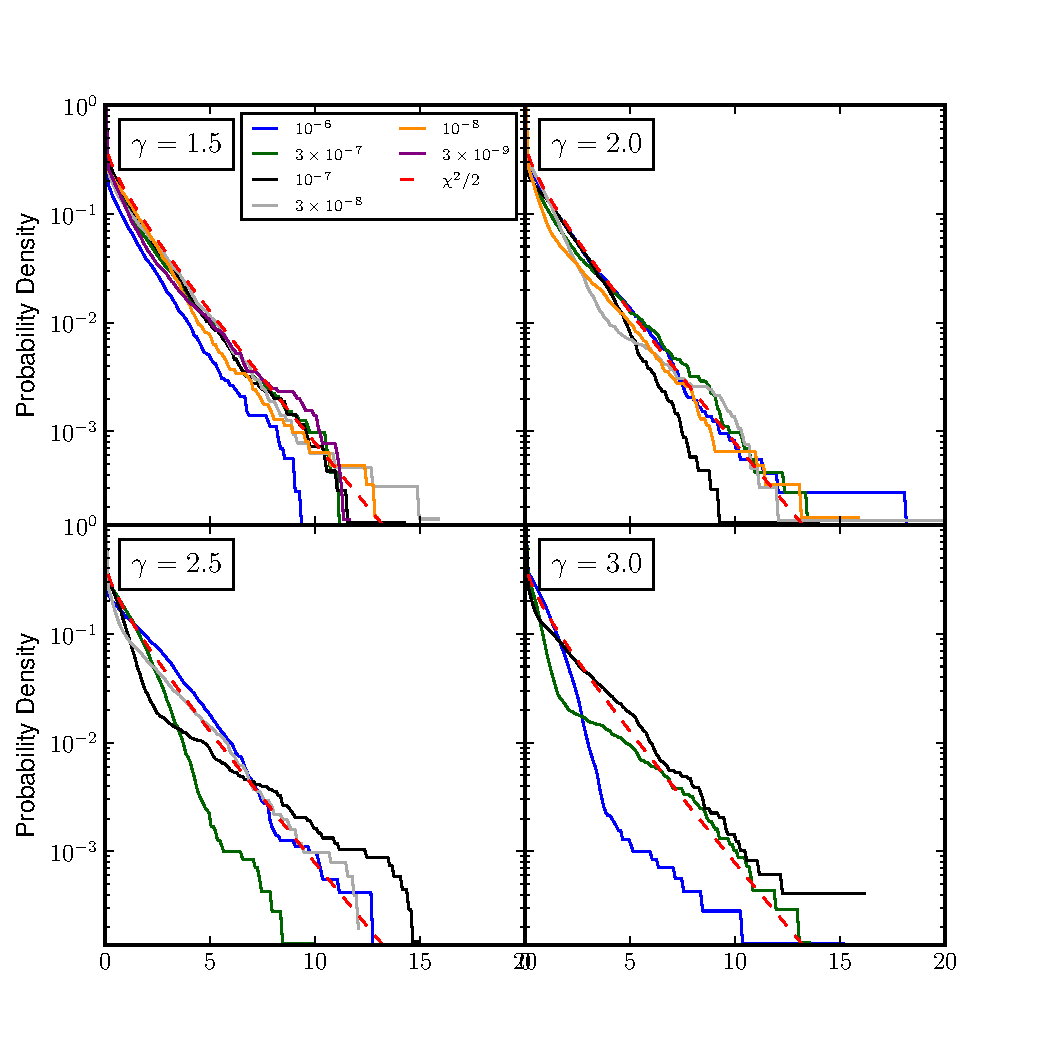
\includegraphics{mc_plots/ts_ext_emin_1000.pdf}
    % this plot came from /u/gl/lande/work/fermi/extended_catalog/monte_carlo/ts_ext/v3/plot.py
    % using data from /nfs/slac/g/ki/ki03/lande/extended_catalog/monte_carlo/ts_ext/v3_emin_1000/merged.hdf5
    \end{center}
    \caption{
    The results of the monte carlo simulation described in section
    \ref{monte_carlo_validation} testing the null distribution of
    the likelihood ratio test for extension.  The $x$ axis of this
    plot is \tsext and the $y$ axis is the cumulative density for
    \tsext that was found by testing simulated point sources of
    various spectral models for extension. The four plots represent
    different spectral indices (for $\gamma$ of 1, 2, 2.5, and 3).
    And the different colors lines represent different fluxes chosen
    to span a representative range of Overlayed on the plot in dashed
    red is the cumulative density function of $\chi^2(\ts)/2$ which is
    suggested by Wilks' theorem as the theoretical distribution these
    curves should should follow.  Overall, it should be noted that there
    is a surprisingly good agreement between the monte carlo study and
    the theoeretical distribution. And for most spectral parameters, the
    Monte Carlo curve lies to the left of the theoretical curve, which
    would imply that using Wilks' Theorem as the null distribution would
    conservativly underestimate the signifcance of a source detection. In
    the rest of the paper, we use this theoretical curve to estimate
    the significance of our source detections.  What is quoted is the
    $>100\mev$ integral flux in measured in units of $\ph/\cm^2/\s$.
    For each spectral model, more information about the simulations is
    summarized in table~\ref{ts_ext_num_sims}. More
    information about this monte carlo analysis is presented in
    section~\ref{monte_carlo_validation}
    }\label{ts_ext_mc}
  \end{figure}

\clearpage

\begin{figure}
  \begin{center}
    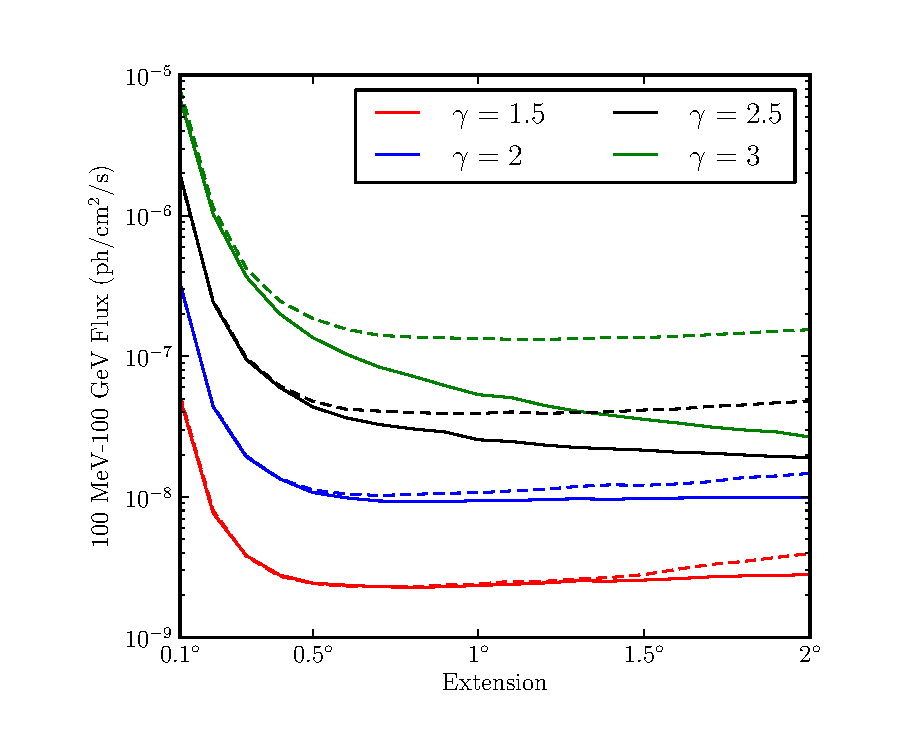
\includegraphics{mc_plots/index_sensitivity.pdf}
    % this plot came from /u/gl/lande/work/fermi/extended_catalog/monte_carlo/sensitivity/v9/plot_vs_index.py
    \end{center}
    \caption{This is the Fermi LAT's sensitivity to spatially
    extended sources. The $x$ axis is Monte Carlo extension of a
    simulated uniform disk source and the $y$ axis is the simulated
    source's $100\mev$ to $100\gev$ photon flux. Each curve represents
    the detection threshold for being able to spatially resolve an
    extended source (when $\langle\tsext\rangle=25$ averaged over
    multiple simulations).  
    All sources have an assumed powerlaw spectrum and the different
    colors are for sources of different simulated spectral indices.
    The dashed line shows simulations using events with energy between 
    $100\mev$ and $100\gev$ while the solid lien shows simulations
    using events with energy between $1\gev$ and $100\gev$.
    The sensitivity is for a one year simulation against a Sreekumar-like
    isotropic background\cite{Sreekumar et al. ApJ 494 pag 523 1998}.
    This plot shows that our sensitivity is best for sources that are
    about $1\deg$ large. It also shows that for sources That are neither
    very large nor very soft, our sensitivity is not significantly
    improved using events between $100\mev$ and $1\gev$.  More information
    about this plot is presented in section~\ref{extension_sensitivity}.
    }\label{index_sensitivity}
  \end{figure}

\clearpage

\begin{figure}
  \begin{center}
    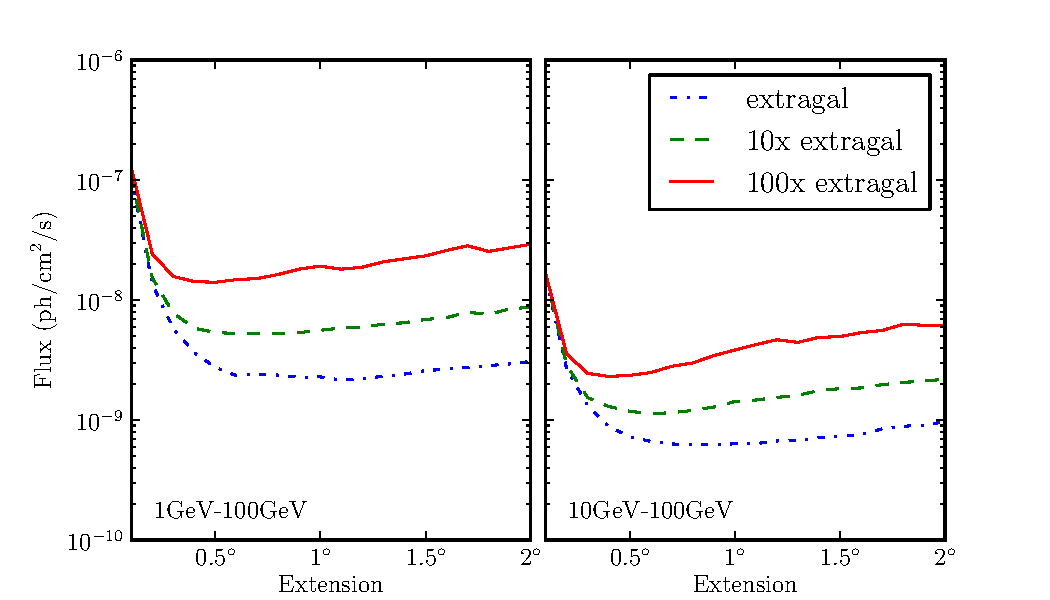
\includegraphics{mc_plots/diff_factor_sensitivity.pdf}
    % this plot came from /u/gl/lande/work/fermi/extended_catalog/monte_carlo/sensitivity/v9/plot_vs_diff_factor.py
    \end{center}
    \caption{Lalla}\label{diff_factor_sensitivity}
  \end{figure}

  \begin{figure}
    \begin{center}
      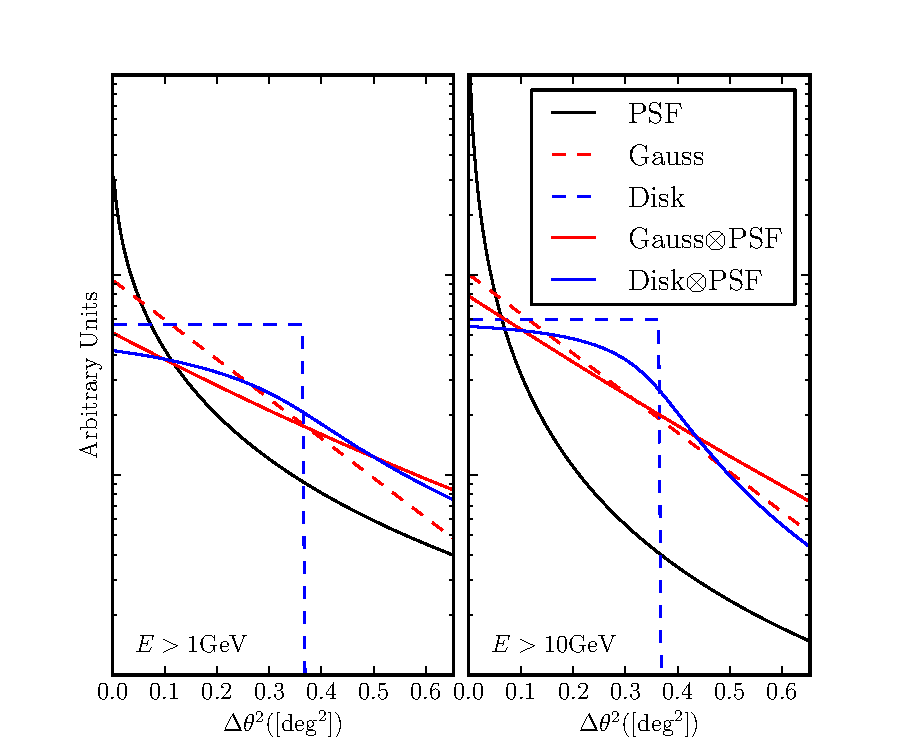
\includegraphics{mc_plots/compare_disk_gauss.pdf}
      % this plot came from /u/gl/lande/work/fermi/extended_catalog/2FGL/plots_for_paper/compare_disk_gauss/v2/compare_disk_gauss.pdf
    \end{center}
    \caption{Comparison of Disk and Gauss.
    % XXXXXXXXXXXXXXXXXXXXX
    % the overall point here is that disk looks like gauss once convolved with the psf.
    }\label{compare_disk_gauss}
  \end{figure}

  \begin{figure}
    \begin{center}
      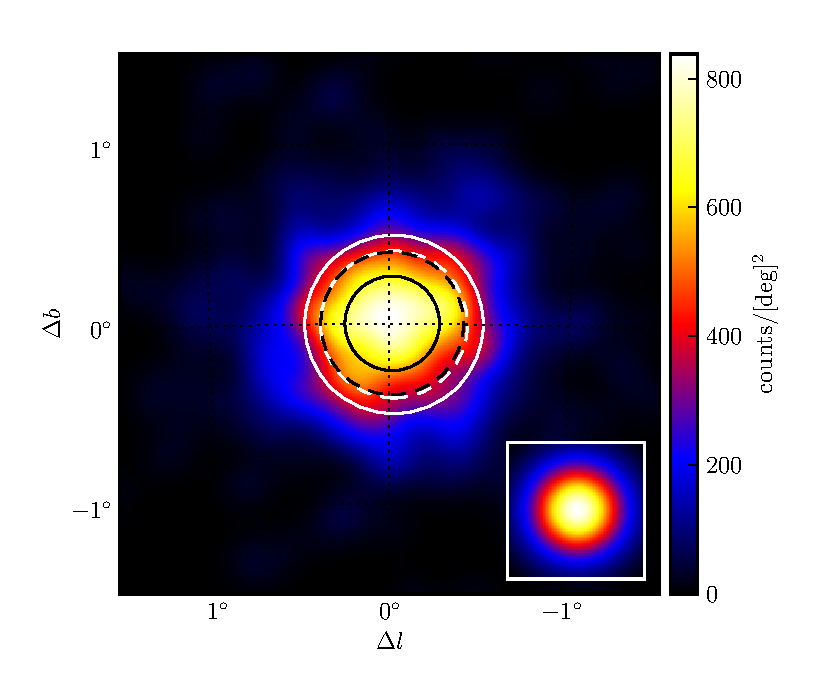
\includegraphics{mc_plots/compare_r68.pdf}
      % this plot came from /u/gl/lande/work/fermi/extended_catalog/2FGL/plots_for_paper/compare_r68/v2/plot.py
    \end{center}
    \caption{Comparison of r68 for disk and gauss. This is a simulated disk source.
    % XXXXXXXXXXXXXXXXXXXXX
    % Add more to caption about htis plot.
    }\label{compare_r68}
  \end{figure}

\begin{figure}
  \begin{center}
    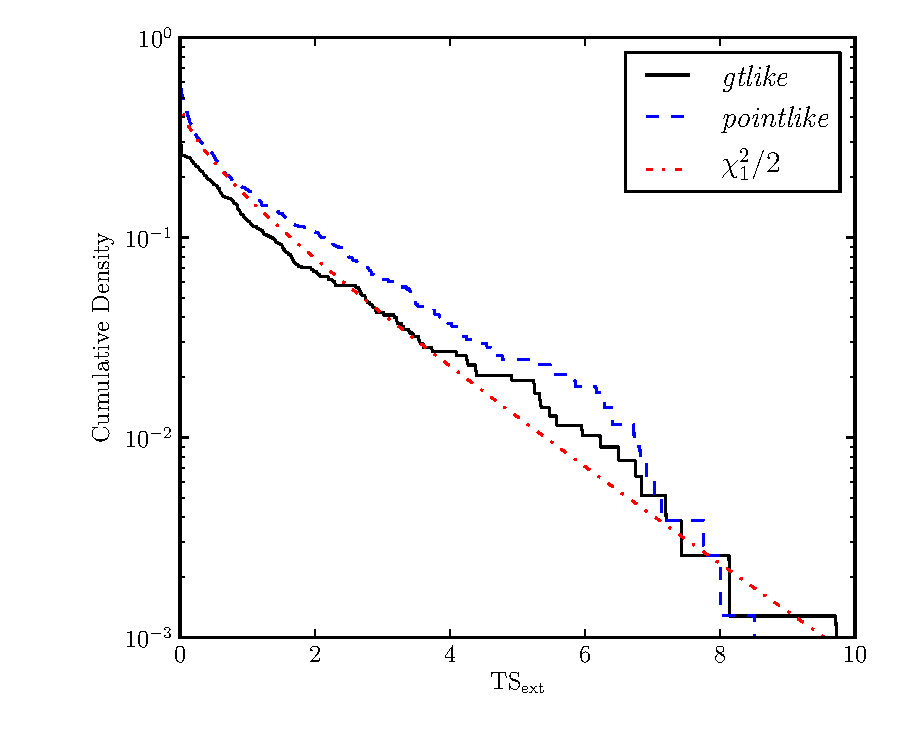
\includegraphics{source_plots/agn.pdf}
    % this plot came from /u/gl/lande/work/fermi/extended_catalog/2FGL/agn/v2/agn.py
    \end{center}
    \caption{Lalla
% XXXXXXXXXXXXXXXXXXXXXXXXXXXXXXXXXXXXXXXXXXXXXX
% Note about how TSext for AGN calculated with pointlike
    }\label{agn_ts_ext}
  \end{figure}


\begin{figure}
  \begin{center}
  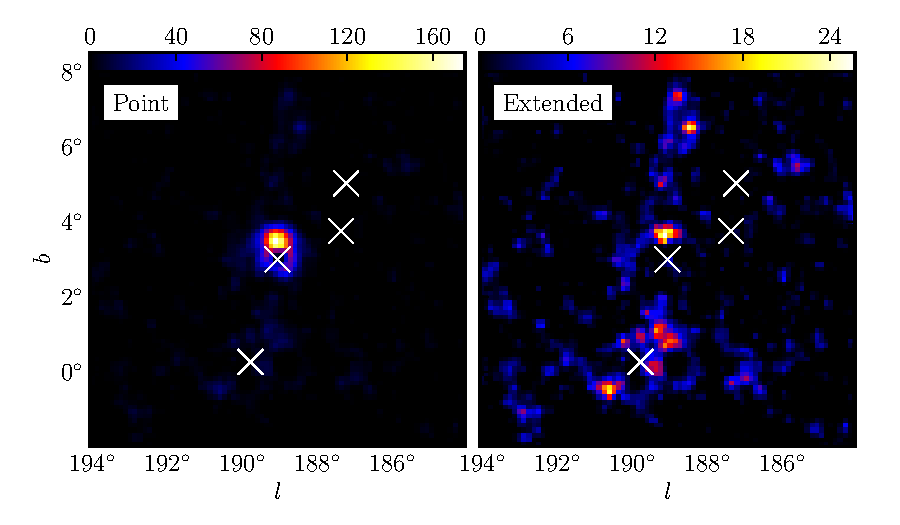
\includegraphics{ic443_plots/res_tsmap_ic443.pdf}
  % plot from /u/gl/lande/work/fermi/extended_catalog/2FGL/plots_for_paper/res_tsmap_ic443/v1

  \caption{An example residual test statistic map generated for the
  supernova rememnant IC443 using events between $1\gev$ and
  $100\gev$.  The top plot is the residual TS map fitting IC443
  as a point source and the bottom plot is the residual TS map fitting
  IC443 as an extended source. The crosses in the plot represent all of
  the sources fit in the region. Since there is a residual TS greater
  than 160 fitting with the point hypothesis, it is clear that a point
  source is not a good fit to the region. On the other hand,
  the residual TS fitting as an extended source is much lower, showing
  that IC443 is better fit by an extended source. These plots were generated
  for all extended source candidates to help validate the analysis.}
  \label{res_tsmaps}
  \end{center}
\end{figure}

\clearpage
\begin{figure}
  \begin{center}
    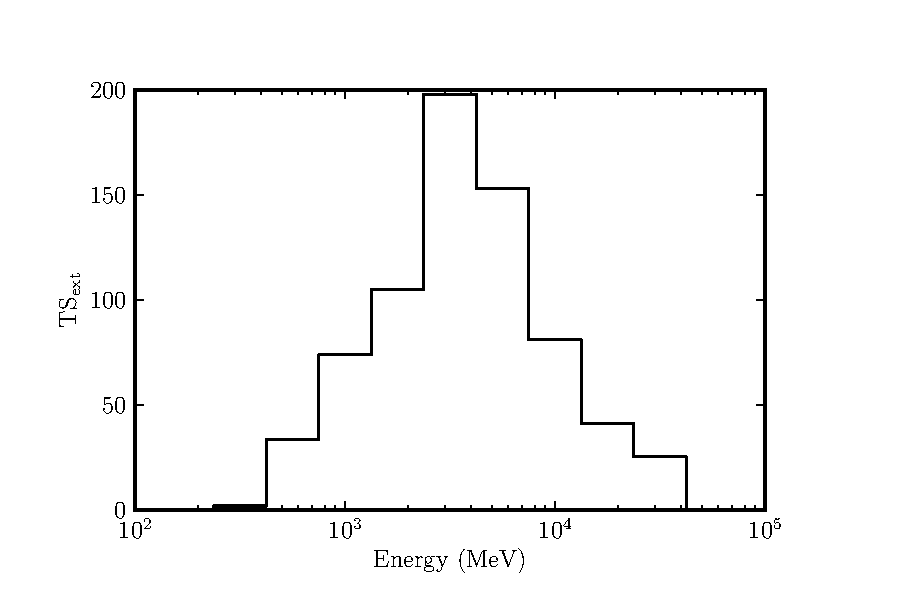
\includegraphics{ic443_plots/ic443_ts_ext_vs_energy.pdf}
    % taken from /u/gl/lande/work/fermi/extended_catalog/2FGL/plots_for_paper/ts_ext_vs_energy/v1/ts_ext_vs_energy.py
    \caption{A plot of \tsext vs log(energy)
    for the SNR IC443, which has a typical spectral model.}
    \label{ts_ext_vs_energy}
  \end{center}
\end{figure}

\clearpage
\begin{figure}
  \begin{center}
    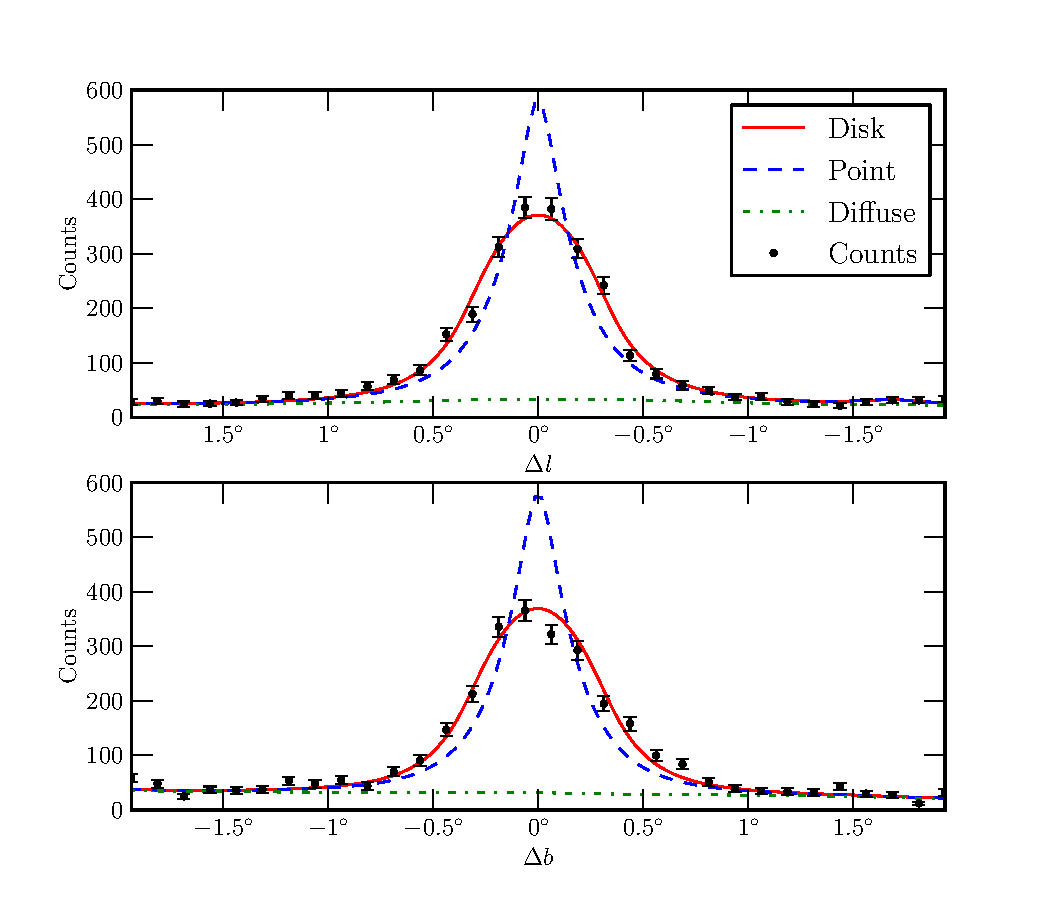
\includegraphics{ic443_plots/ic443_counts_slice.pdf}
    % taken from /u/gl/lande/work/fermi/extended_catalog/2FGL/plots_for_paper/counts_slice_ic443/v1/ic443_counts_slice.pdf
    \caption{
    % XXXXXXXXXXXXXXXXXXXXXXXXXXXXX
    % best for lookign at overall diffuse emission and visually assesing quality of the fit.
    }
    \label{counts_slice}
  \end{center}
\end{figure}

\clearpage
\begin{figure}
  \begin{center}
    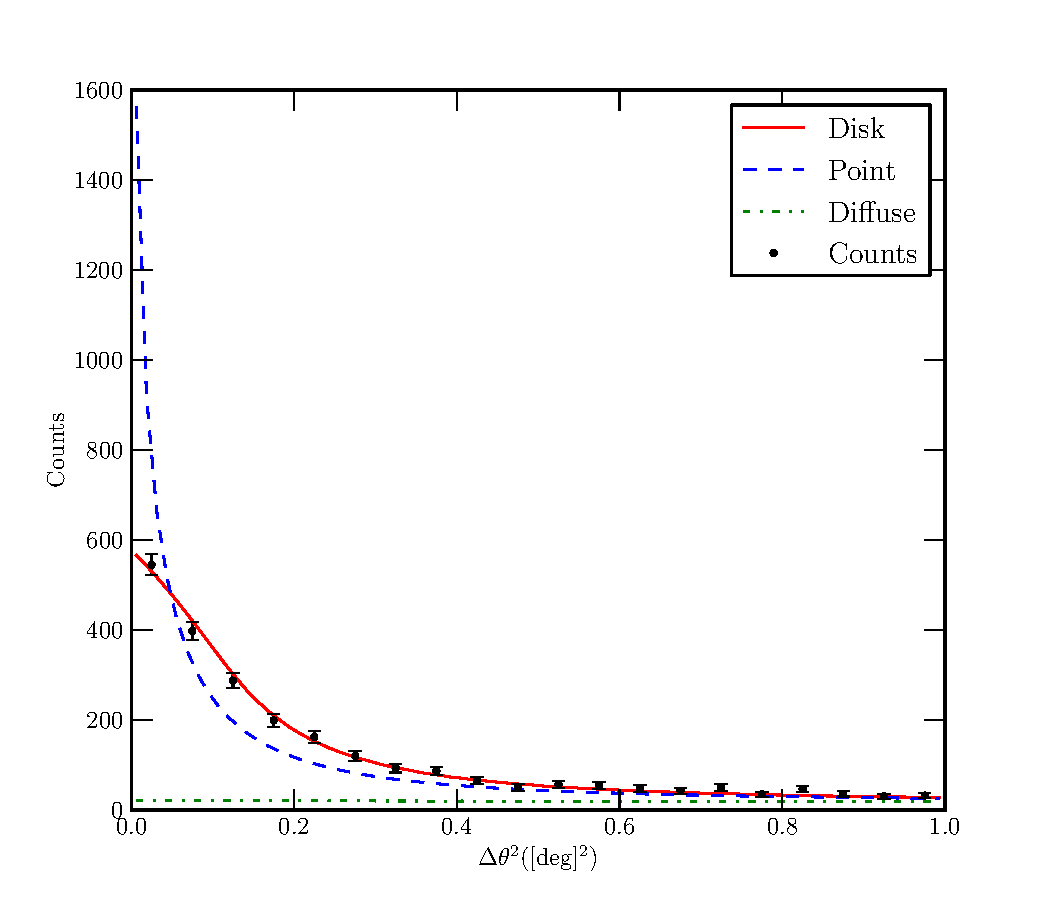
\includegraphics{ic443_plots/ic443_radial_integral.pdf}
    % taken from /u/gl/lande/work/fermi/extended_catalog/2FGL/plots_for_paper/radial_integral_ic443/v1/ic443_radial_integral.pdf
    \caption{The radial integral of the counts and the model predicted counts.}
    \label{radial_profile}
  \end{center}
\end{figure}

\clearpage
\begin{figure}
  \begin{center}
    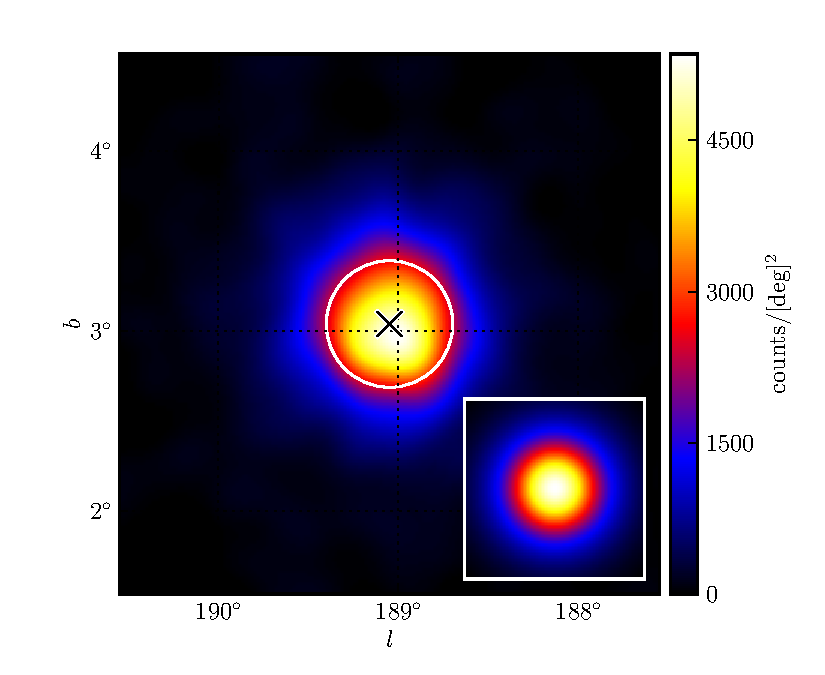
\includegraphics{ic443_plots/ic443_smoothed_counts.pdf}
    % taken from /u/gl/lande/work/fermi/extended_catalog/2FGL/plots_for_paper/smoothed_counts_ic443/v1
    \caption{Smoothed counts. Galactic and isotoropic as well as earth albedo background were subtracted.
    % XXXXXXXXXXXXXXXXXXXXXXXXXXX 
    % describe that this is IC443 using (front? or back? or both?) events.
    }
    \label{smoothed_counts}
  \end{center}
\end{figure}

% XXXXXXXXXXXXXXXXXXXXXXXX
% Make IC443 extension profile
% good for looking for
% how peaky likelihood is and
% wheter or not there is one unique
% extension maximum (Often times
% double peaked or does not fall
% at low/high energies.
% 
\clearpage
\begin{figure}
  \begin{center}
    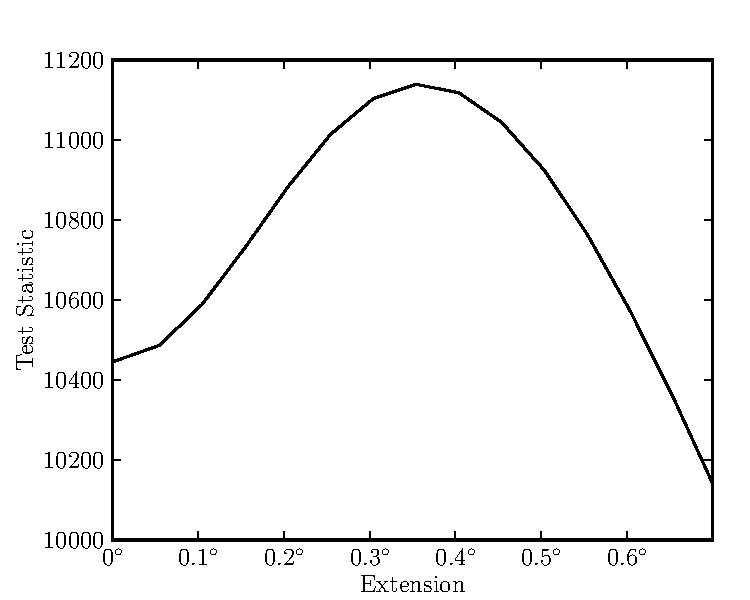
\includegraphics{ic443_plots/profile_ic443.pdf}
    % taken from /u/gl/lande/work/fermi/extended_catalog/2FGL/plots_for_paper/extension_profile_ic443/v1/profile_ic443.pdf
    \caption{Smoothed counts. Galactic and isotoropic as well as earth albedo background were subtracted.
    % XXXXXXXXXXXXXXXXXXXXXXXXXXX 
    % describe that this is IC443 using (front? or back? or both?) events.
    }
    \label{extension_profile}
  \end{center}
\end{figure}



% XXXXXXXXXXXXXXXXXXXXXXX
% example bad fit
% P72Y3047

\clearpage
\begin{sidewaystable}
    \begin{centering}
      \begin{tabular}{r|rrrrrrrrrr}
        \hline
        \hline
        Name                 &          \glon &          \glat &                    $\sigma$ &       TS &   $\tsext$ &      Major &      Minor &    Pos Ang &      Flux ($10^{-9}$) &                 Index \\
        \hline
        \multicolumn{11}{c}{$E > 1\gev$} \\
        \hline
        SMC                  &     302.87\deg &     -44.65\deg & $  1.59\deg \pm   0.15\deg$ &     93.1 &       51.2 &  0.173\deg &  0.129\deg &   41.9\deg & $    3.0 \pm     0.4$ & $   2.42 \pm    0.16$ \\
        LMC                  &     278.58\deg &     -32.82\deg & $  2.26\deg \pm   0.09\deg$ &    384.2 &      304.4 &  0.096\deg &  0.071\deg &  -35.5\deg & $   12.9 \pm     0.7$ & $   2.42 \pm    0.08$ \\
        IC443                &     189.05\deg &       3.04\deg & $  0.35\deg \pm   0.01\deg$ &  10765.3 &      535.3 &  0.006\deg &  0.006\deg &   84.0\deg & $   65.2 \pm     1.2$ & $   2.23 \pm    0.02$ \\
        W28                  &       6.51\deg &      -0.29\deg & $  0.39\deg \pm   0.02\deg$ &   1231.3 &       92.1 &  0.014\deg &  0.013\deg &   30.4\deg & $   55.9 \pm     1.8$ & $   2.65 \pm    0.03$ \\
        W30                  &       8.61\deg &      -0.20\deg & $  0.36\deg \pm   0.04\deg$ &    458.1 &       66.0 &  0.020\deg &  0.018\deg &   14.1\deg & $   30.0 \pm     1.8$ & $   2.58 \pm    0.06$ \\
        W44                  &      34.68\deg &      -0.42\deg & $  0.34\deg \pm   0.02\deg$ &   1387.6 &      111.3 &  0.009\deg &  0.009\deg &  -39.4\deg & $   74.7 \pm     1.0$ & $   2.67 \pm    0.01$ \\
        W51C                 &      49.12\deg &      -0.44\deg & $  0.28\deg \pm   0.02\deg$ &   2174.7 &       87.6 &  0.010\deg &  0.010\deg &   59.4\deg & $   41.6 \pm     1.3$ & $   2.38 \pm    0.04$ \\
        \hline
        \multicolumn{11}{c}{$E > 10\gev$} \\
        \hline
        HESS J1825-137       &      17.58\deg &      -0.46\deg & $  0.64\deg \pm   0.08\deg$ &     85.6 &       62.5 &  0.050\deg &  0.045\deg &   33.6\deg & $    1.8 \pm     0.3$ & $   1.75 \pm    0.20$ \\
        MSH 15-52            &     320.39\deg &      -1.22\deg & $  0.20\deg \pm   0.06\deg$ &     73.7 &        9.5 &  0.033\deg &  0.032\deg &    3.9\deg & $    0.6 \pm     0.1$ & $   2.32 \pm    0.23$ \\

      \end{tabular}
      \caption{The fit results for the already known extended sources that
      were found by our analysis. The top results were found using an
      energy range between $1\gev$ and $100\gev$.  The lower analysis
      was done using events between $10\gev$ and $100\gev$.  The quoted
      flux is in units of $10^{-9}\ph/\cm^2/\s$ and is the flux in the
      fit energy range (either 1\gev to 100\gev or 10\gev to 100\gev).
      All sources were fit using a uniform disk spatial template. The
      localization and extension were found using \pointlike while the
      TS and spectral values were calculated using \gtlike.  The TS value
      was computed using the assumed disk morphology and \tsext compares
      is the increase in \ts fitting the source with an extended spatial
      model instead of a point model.  \glon and \glat are respectivly
      the galactic longitute and galactic latitude of the source and
      $\sigma$ is the edge of the uniform disk spatial model that was fit
      to the source.  The Centaurus A Lobes, the Cygnus Loop, and Vela
      X were not found to be extended by this too. The
      reasons for this are discussed in section~\ref{validate_known}.
      }
      \label{known_extended_sources}
    \end{centering}
\end{sidewaystable}


\clearpage

\begin{sidewaystable}
  \begin{centering}
    \begin{tabular}{r|rrrrrrrrrr}
      \hline
      \hline
      Name                 &          \glon &          \glat &                    $\sigma$ &       TS &   $\tsext$ &      Major &      Minor &    Pos Ang &      Flux ($10^{-9}$) &                 Index \\
      \hline
      \multicolumn{11}{c}{$E > 1\gev$} \\
      \hline
      P72Y2516             &     353.08\deg &      16.80\deg & $  0.41\deg \pm   0.05\deg$ &    139.2 &       28.9 &  0.042\deg &  0.036\deg &   54.4\deg & $    6.3 \pm     0.6$ & $   2.50 \pm    0.14$ \\
      P72Y2405             &     328.13\deg &       0.26\deg & $  0.49\deg \pm   0.04\deg$ &    148.8 &       77.6 &  0.046\deg &  0.041\deg &   55.3\deg & $   16.2 \pm     1.5$ & $   2.31 \pm    0.11$ \\
      P72Y1212             &     260.31\deg &      -3.28\deg & $  0.37\deg \pm   0.03\deg$ &    314.6 &       49.2 &  0.026\deg &  0.023\deg &    5.0\deg & $    8.3 \pm     0.3$ & $   2.18 \pm    0.02$ \\
      \hline
      \multicolumn{11}{c}{$E > 10\gev$} \\
      \hline
      P72Y2473             &     331.74\deg &      -0.58\deg & $  0.52\deg \pm   0.04\deg$ &     75.3 &       45.2 &  0.071\deg &  0.049\deg &  -21.9\deg & $    1.3 \pm     0.2$ & $   1.75 \pm    0.25$ \\
      P72Y2540             &     336.52\deg &       0.06\deg & $  0.65\deg \pm   0.03\deg$ &    173.0 &       95.3 &  0.041\deg &  0.037\deg &    5.3\deg & $    2.9 \pm     0.2$ & $   2.28 \pm    0.08$ \\
      P72Y3281             &      78.33\deg &       2.22\deg & $  0.71\deg \pm   0.04\deg$ &    245.7 &      151.7 &  0.047\deg &  0.038\deg &    4.3\deg & $    2.1 \pm     0.2$ & $   2.36 \pm    0.18$ \\
      P72Y2979             &      25.09\deg &       0.13\deg & $  0.35\deg \pm   0.07\deg$ &     47.3 &       20.6 &  0.076\deg &  0.063\deg &   -7.7\deg & $    1.0 \pm     0.2$ & $   1.59 \pm    0.30$ \\
      P72Y1287             &     266.29\deg &      -1.43\deg & $  1.15\deg \pm   0.08\deg$ &    119.6 &       90.9 &  0.080\deg &  0.065\deg &   54.6\deg & $    1.3 \pm     0.2$ & $   1.76 \pm    0.18$ \\
      \hline
    \end{tabular}
    \caption{This table presents the new extended soruce candidates found with
    this search. 3 new extended sources were found searching above 1\gev and
    5 new candidates were found looking above 10\gev.
    The columns in this table have the same defintion as table~\ref{known_extended_sources}.}
    \label{new_ext_srcs}
  \end{centering}
\end{sidewaystable}


\clearpage
\begin{sidewaystable}
    \begin{centering}
      \begin{tabular}{r|rr|rrrr|rrrr}
        \hline
        \hline
        Name                 &     \tsinc &     \tsext &      $\glon_1$ &      $\glat_1$ & $\text{Flux}_1$ ($10^{-9}$) &   $\text{Index}_1$ &      $\glon_2$ &      $\glat_2$ & $\text{Flux}_1$ ($10^{-9}$) &  $\text{Index}_2$ \\
        \hline
        \multicolumn{11}{c}{$E > 1\gev$} \\
        \hline
        P72Y2516             &       23.8 &       28.9 &     353.04\deg &      16.96\deg & $       3.5 \pm        0.6$ & $  2.7 \pm   0.3$  &     353.14\deg &      16.50\deg & $       2.0 \pm        0.5$ & $  2.4 \pm   0.3$ \\
        P72Y2405             &       48.6 &       77.6 &     328.31\deg &       0.31\deg & $      10.0 \pm        1.2$ & $  2.7 \pm   0.2$  &     328.28\deg &      -0.06\deg & $       1.0 \pm        0.7$ & $  1.6 \pm   0.4$ \\
        P72Y1212             &       22.2 &       49.2 &     260.59\deg &      -3.26\deg & $       2.0 \pm        0.5$ & $  1.9 \pm   0.2$  &     260.24\deg &      -3.20\deg & $       5.3 \pm        0.6$ & $  2.4 \pm   0.1$ \\
        \hline
        \multicolumn{11}{c}{$E > 10\gev$} \\
        \hline
        P72Y2473             &       34.3 &       45.2 &     331.77\deg &      -0.35\deg & $       0.3 \pm        0.1$ & $  1.1 \pm   0.5$  &     331.51\deg &      -0.83\deg & $       0.4 \pm        0.1$ & $  2.1 \pm   0.5$ \\
        P72Y2540             &       24.8 &       95.3 &     336.16\deg &       0.34\deg & $       0.7 \pm        0.1$ & $  2.0 \pm   0.4$  &     336.72\deg &      -0.06\deg & $       0.7 \pm        0.1$ & $  3.1 \pm   0.5$ \\
        P72Y3281             &       34.5 &      151.7 &      78.08\deg &       2.53\deg & $       0.4 \pm        0.1$ & $  2.0 \pm   0.5$  &      78.45\deg &       2.54\deg & $       0.5 \pm        0.1$ & $  1.9 \pm   0.4$ \\
        P72Y2979             &       15.4 &       20.6 &      25.06\deg &       0.24\deg & $       0.3 \pm        0.1$ & $  1.1 \pm   0.6$  &      25.08\deg &      -0.05\deg & $       0.4 \pm        0.1$ & $  1.9 \pm   0.6$ \\
        P72Y1287             &       32.5 &       90.9 &     267.16\deg &      -1.60\deg & $       0.2 \pm        0.1$ & $  1.9 \pm   0.4$  &     266.43\deg &      -1.39\deg & $       0.2 \pm        0.1$ & $  1.5 \pm   0.5$ \\
        \hline
      \end{tabular}
      \label{dual_localization_results}
      \caption{For the new extended source candidates in
      figure~\ref{new_ext_srcs}, we describe the results
      of the dual localization procedure described in
      section~\ref{dual_localization_method}. Here, the extended
      source candidate is not fit as an extended source but instead
      fit as two point sources.  The dual localization is performed
      with \pointlike and results in the best fit position of the two
      sources $(\glon_1,\glat_1)$ and $(\glon_2,\glat_2)$.  The change in
      likelihood and spectral values are then computed using \gtlike with
      the best fit positions found by \pointlike.  \tsinc is the increase
      in TS fitting the region as two sources compared to fitting compared
      to fitting a single point source and is computed using \gtlike with
      the best fit positions taken from \pointlike.  It can be directly
      compared to \tsext, which is taken from table \ref{new_ext_srcs}.
      For all of our candiates, $\tsext > \tsinc$ which shows that an
      extended source fits the source better than two point sources.
      As in table~\ref{known_extended_sources}, flux is measured in
      units of $10^{-9}\ph/\cm^2/\s$ and is the integral flux between
      1\gev (10\gev) and 100\gev for the sources found using events above 1\gev (10\gev).
      }
    \end{centering}
  \end{sidewaystable}


  \clearpage
  \begin{sidewaystable}
    \begin{centering}
      \begin{tabular}{r|rrrrrrrr}
        \hline
        \hline
        Name                 &     $\ts_\pointlike$ &        $\ts_\gtlike$ &           $\ts_\alt$ &          \tsextpointlike &           \tsextgtlike &            \tsextalt &                    $\sigma$ &               $\sigma_\alt$ \\
        \hline
        \multicolumn{9}{c}{$E > 1\gev$} \\
        \hline
        P72Y2516             &                155.0 &                139.2 &                103.8 &                     38.5 &                   28.9 &                 22.5 & $  0.41\deg \pm   0.05\deg$ & $  0.38\deg \pm   0.04\deg$ \\
        P72Y2405             &                108.4 &                148.8 &                138.4 &                     25.7 &                   77.6 &                 40.6 & $  0.49\deg \pm   0.04\deg$ & $  0.51\deg \pm   0.04\deg$ \\
        P72Y1212             &                329.5 &                314.6 &                345.6 &                     60.4 &                   49.2 &                 51.5 & $  0.37\deg \pm   0.03\deg$ & $  0.38\deg \pm   0.03\deg$ \\
        \hline
        \multicolumn{9}{c}{$E > 10\gev$} \\
        \hline
        P72Y2473             &                 74.7 &                 75.3 &                 88.7 &                     43.7 &                   45.2 &                 50.0 & $  0.52\deg \pm   0.04\deg$ & $  0.53\deg \pm   0.03\deg$ \\
        P72Y2540             &                173.9 &                173.0 &                157.7 &                     97.9 &                   95.3 &                 93.6 & $  0.65\deg \pm   0.03\deg$ & $  0.66\deg \pm   0.03\deg$ \\
        P72Y3281             &                244.9 &                245.7 &                264.3 &                    152.8 &                  151.7 &                162.9 & $  0.71\deg \pm   0.04\deg$ & $  0.71\deg \pm   0.03\deg$ \\
        P72Y2979             &                 43.4 &                 47.3 &                 39.0 &                     17.4 &                   20.6 &                 17.7 & $  0.35\deg \pm   0.07\deg$ & $  0.34\deg \pm   0.06\deg$ \\
        P72Y1287             &                117.1 &                119.6 &                124.7 &                     86.1 &                   90.9 &                 95.0 & $  1.15\deg \pm   0.08\deg$ & $  1.16\deg \pm   0.08\deg$ \\
        \hline
      \end{tabular}
      \label{alt_diff_model_results}
      \caption{
      This table shows a comparison of the \ts values gotten using \gtlike and \pointlike.
      It also compares the fit values using the standard diffuse model and using the alternate
      diffuse model described in section~\ref{alt_diff_model_description}.
      $\ts_\pointlike$ is the \ts of the source fit with the extended hypothesis using \pointlike
      whereas $\ts_\gtlike$ is the same quantity using the same model but fitting with \gtlike.
      There is very good agreement between the two methods.
%&        $\ts_\gtlike$ &           $\ts_\alt$ &          \tsextpointlike &           \tsextgtlike &            \tsextalt &                    $\sigma$ &               $\sigma_\alt$ \\
      }
    \end{centering}
  \end{sidewaystable}


\begin{figure}
  \begin{center}
    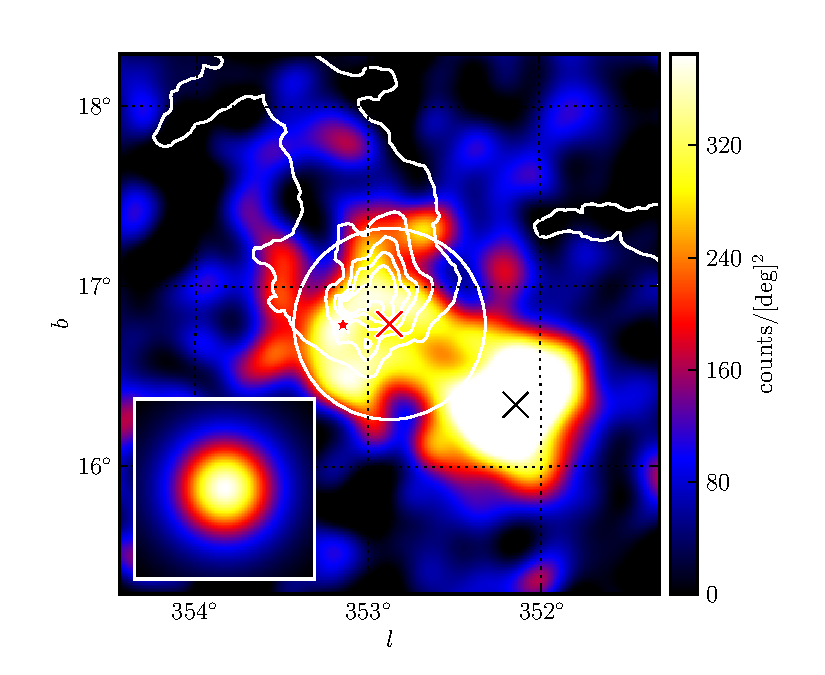
\includegraphics[type=pdf,ext=.pdf,read=.pdf]{source_plots/source_1FGL_J1628.6-2419c}
  \end{center}
  % this plot came from 
  % /u/gl/lande/work/fermi/extended_catalog/2FGL/plots_for_paper/source_plots/1FGL_J1628.6-2419c/v2/run.py
  \caption{1FGL J1628.6-2419c. In the opiucus region=most likeliy a molecular cloud.
  P72Y2516.
  Note that unlike other plots, that this plot has the nearby sources subtracted.
  This was done to remove the very bright, $\ts=460$, source P72Y2510 % XXXXXXXXXXXXXXXXXXXX what is this source
  which would be in the lower right of the image at $l,b=352.14\deg,16.34\deg$.
  }\label{1FGL_J1628.6-2419c}
\end{figure}

\begin{figure}
  \begin{center}
    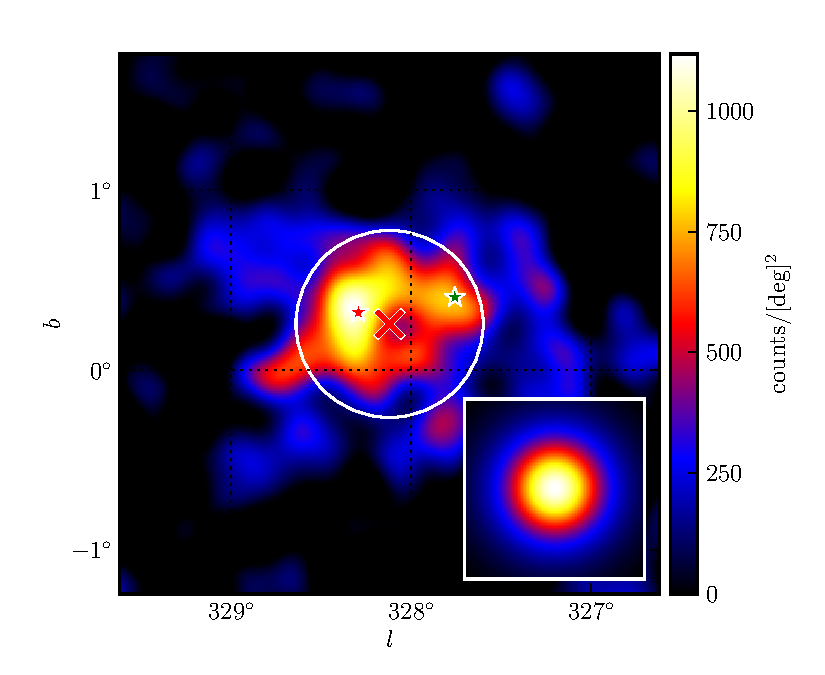
\includegraphics[type=pdf,ext=.pdf,read=.pdf]{source_plots/source_1FGL_J1554.0-5345c}
  \end{center}
  % this plot came from 
  % /u/gl/lande/work/fermi/extended_catalog/2FGL/plots_for_paper/source_plots/1FGL_J1554.0-5345c/v2/source_1FGL_J1554.0-5345c.pdf
  \caption{1FGL J1554.0-5345c. P72Y2405. Unidentified source likely diffuse emission.}
  \label{1FGL_J1554.0-5345c}
\end{figure}

\begin{figure}
  \begin{center}
    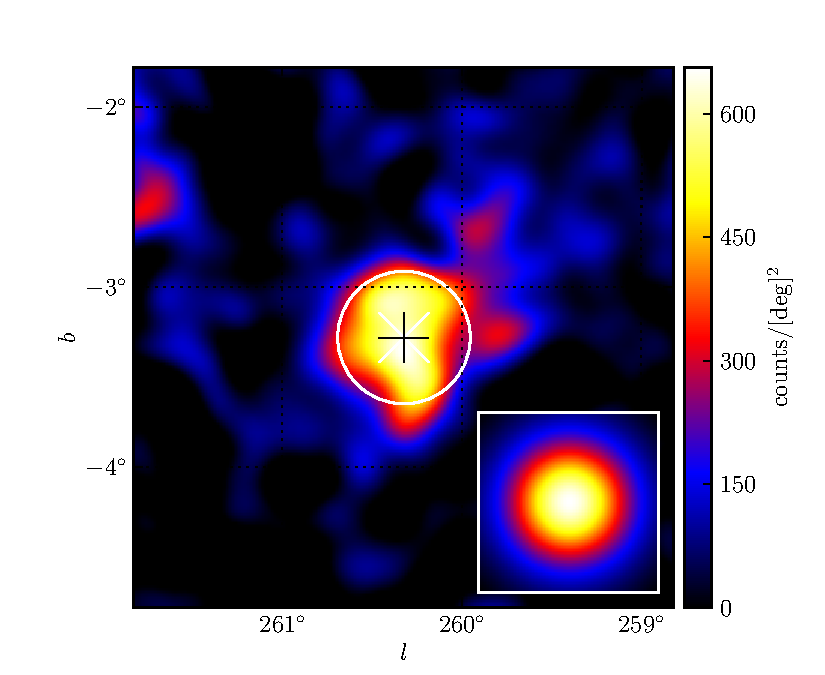
\includegraphics[type=pdf,ext=.pdf,read=.pdf]{source_plots/source_1FGL_J0823.3-4248}
  \end{center}
  % this plot came from 
  % /u/gl/lande/work/fermi/extended_catalog/2FGL/plots_for_paper/source_plots/1FGL_J0823.3-4248/v2/source_1FGL_J0823.3-4248.pdf
  \caption{1FGL J0823.3-4248. P72Y1212. Coincident with Puppis A SNR.
  P72Y1212.
  Note that unlike most other plots, this plot has the nearby sources subtracted.
  This was done to remove the very bright source Vela which,
  at position $l,b=263.55\deg,-2.79\deg$ is over 3 degrees away,
  would otherwise spill over into the top left of the image.
  % XXXXXXXXXXXXXXXXXXXXXXXXXXX add in contour
  }\label{1FGL_J0823.3-4248}
\end{figure}

\begin{figure}
  \begin{center}
    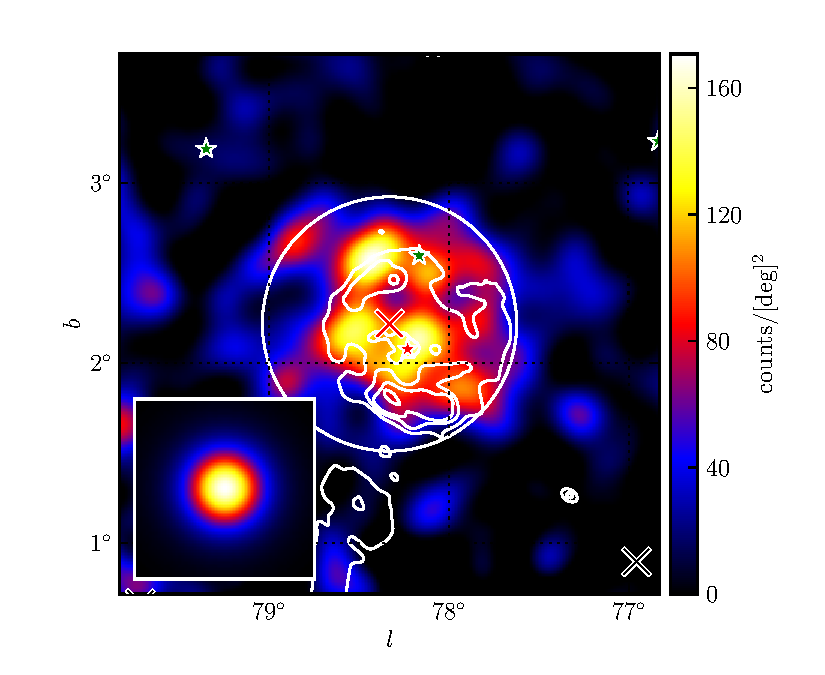
\includegraphics[type=pdf,ext=.pdf,read=.pdf]{source_plots/source_Gamma_Cygni}
  \end{center}
  % this plot came from 
  % /u/gl/lande/work/fermi/extended_catalog/2FGL/plots_for_paper/source_plots/Gamma_Cygni/v2/source_Gamma_Cygni.pdf
  \caption{
  Gamma Cygni. P72Y3281
  }\label{Gamma_Cygni}
\end{figure}

\begin{figure}
  \begin{center}
    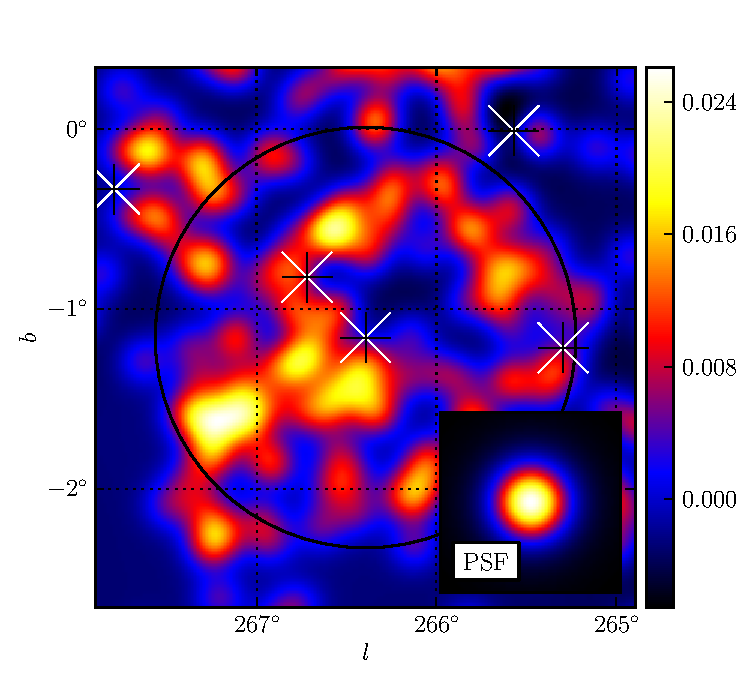
\includegraphics[type=pdf,ext=.pdf,read=.pdf]{source_plots/source_Vela_Jr}
  \end{center}
  % this plot came from 
  % /u/gl/lande/work/fermi/extended_catalog/2FGL/plots_for_paper/source_plots/Vela_Jr/v2/source_Vela_Jr.pdf
  \caption{Vela Jr. P72Y1287. Using $E>10\gev$. Here, the image is
  convovled with a $0.25\deg$ gaussian.
  % XXXXXXXXXXXXXXXXXXXXXXXXXXX add in contour
  }\label{Vela_Jr}
\end{figure}

\begin{figure}
  \begin{center}
    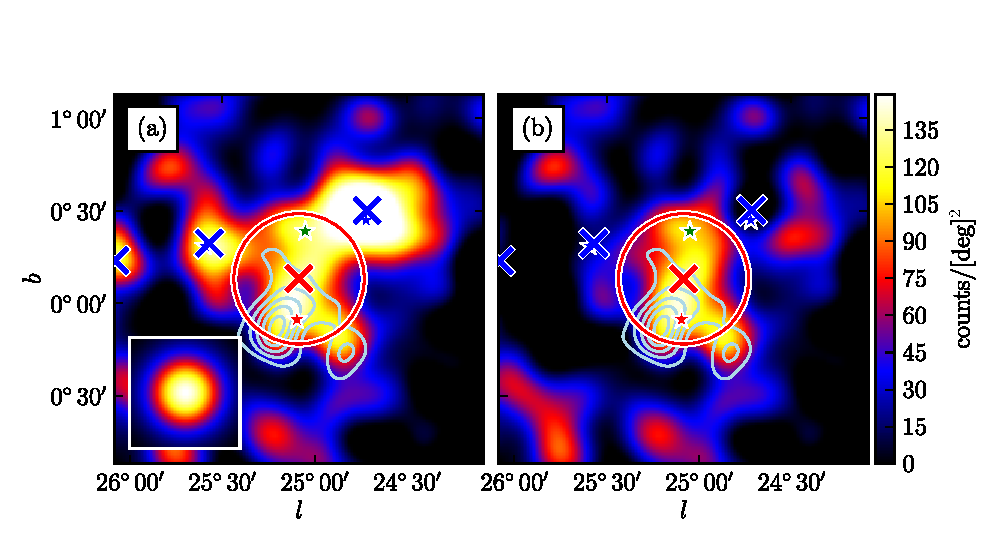
\includegraphics[type=pdf,ext=.pdf,read=.pdf]{source_plots/source_1FGL_J1837.5-0659c}
  \end{center}
  % this plot came from 
  % /u/gl/lande/work/fermi/extended_catalog/2FGL/plots_for_paper/source_plots/1FGL_J1837.5-0659c/v2/source_1FGL_J1837.5-0659c.pdf
  \caption{1FGL J1837.5-0659c. P72Y2974
  % XXXXXXXXXXXXXXXXXXXXXXXXXXX add in contour
  }\label{1FGL_J1837.5-0659c}
\end{figure}


\begin{figure}
  \begin{center}
    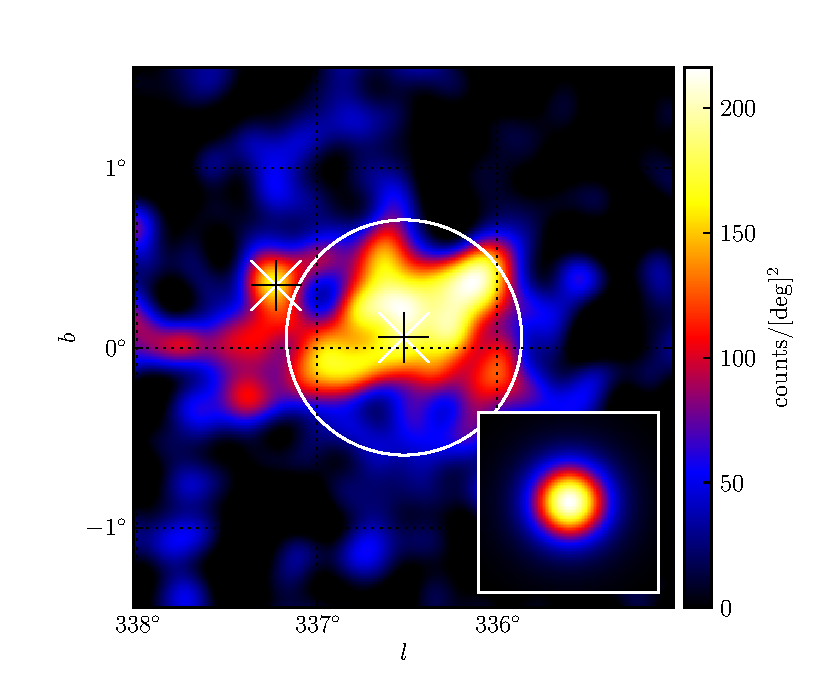
\includegraphics[type=pdf,ext=.pdf,read=.pdf]{source_plots/source_1FGL_J1632.9-4802c}
  \end{center}
  % this plot came from 
  % /u/gl/lande/work/fermi/extended_catalog/2FGL/plots_for_paper/source_plots/1FGL_J1632.9-4802c/v2/source_1FGL_J1632.9-4802c.pdf
  \caption{1FGL J1632.9-4802c. P72Y2540
  % XXXXXXXXXXXXXXXXXXXXXXXXXXX add in contour
  }\label{1FGL_J1632.9-4802c}
\end{figure}


\begin{figure}
  \begin{center}
    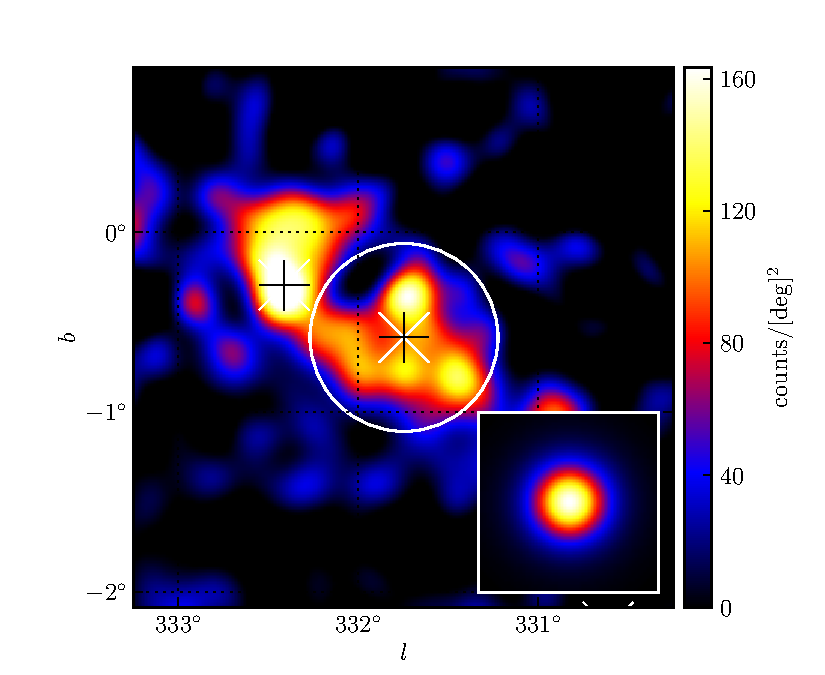
\includegraphics[type=pdf,ext=.pdf,read=.pdf]{source_plots/source_1FGL_J1613.6-5100c}
  \end{center}
  % this plot came from 
  % /u/gl/lande/work/fermi/extended_catalog/2FGL/plots_for_paper/source_plots/1FGL_J1613.6-5100c/v2/source_1FGL_J1613.6-5100c.pdf
  \caption{
  1FGL J1613.6-5100c . P72Y2473
  % XXXXXXXXXXXXXXXXXXXXXXXXXXX add in contour
  }\label{1FGL_J1613.6-5100c}
\end{figure}




\end{document}

